% Template latex non officiel pour rapport de TP EEA.
% C'est un template pour thèse que j'ai adapté et 
% auquel j'ai ajouté des éléments au fil du temps pour mes rapports de TP.
% En cas de problèmes n'hésites pas a me contacter.
% David Tocaven
% david.tocaven@gmail.com


%%% /!\ /!\ /!\ /!\ /!\ /!\
% Se compile avec PDFLatex
%%% /!\ /!\ /!\ /!\ /!\ /!\
%%=================================================%%
%%						MAIN
%%=================================================%%


\documentclass[a4paper]{report}

%====================== PACKAGES ======================
\usepackage{bbold}
\usepackage{soul}				% souligner
\usepackage{dsfont}
\usepackage[french]{babel}		% Pour avoir le document en français
\usepackage[utf8x]{inputenc}	% Encodage du document
\usepackage{float}				% Pour gérer les positionnement d'images
\usepackage{amsmath}
\usepackage{mathrsfs}			% Pour les lettres calligraphiques équation
\usepackage{url}				% Pour faire des hyperliens vers le web
\usepackage{color}
% pour les informations sur un document compilé en PDF et les liens externes / internes
\usepackage{hyperref}			% Pour faire des hyperliens
\usepackage{array}				% Pour faire des tableaux
\usepackage{tabularx}
% pour utiliser 		% floatbarrier
%\usepackage{placeins}
%\usepackage{floatrow}
\usepackage{setspace}			% Espacement entre les lignes
\usepackage{abstract}			% Modifier la mise en page de l'abstract
\usepackage[T1]{fontenc}		% Police et mise en page (marges) du document
\usepackage[top=2cm, bottom=2cm, left=2cm, right=2cm]{geometry}
\usepackage{pdfpages}			% pour inclures des pdf comme des images
\usepackage{subfig}				% Pour les galerie d'images
\usepackage{listings}			% pour inclure du code dans le doc
\usepackage{soul}				% Pour surligner
\usepackage{enumitem}

\sethlcolor{grisclair}
\definecolor{darkgreen}{RGB}{0,100,0}


%====================== INFORMATION ET REGLES ======================

%rajouter les numérotation pour les \paragraphe et \subparagraphe
\setcounter{secnumdepth}{4}
\setcounter{tocdepth}{4}

\hypersetup{							% Information sur le document
pdfauthor = { NOM },				% Auteurs
pdftitle = {Matière - Titre - Sujet },		% Titre du document
pdfsubject = {matière},		% Sujet
pdfkeywords = {},				% Mots-clefs
pdfstartview={FitH}}					% ajuste la page à la largueur de l'écran
%pdfcreator = {MikTeX},% Logiciel qui a crée le document
%pdfproducer = {}} % Société avec produit le logiciel

\newcounter{cpt1}						% Compteur pour les n° de ligne dans les prog de l'annexe1
\newcommand\increm{\arabic{cpt1}\addtocounter{cpt1}{1}}
%initialisation de l'intégrateur de language C



%======================== DEBUT DU DOCUMENT ========================

\begin{document}

%\lstset{
%  language=C,                	  % choose the language of the code
%  numbers=left,                   % where to put the line-numbers
%  stepnumber=1,                   % the step between two line-numbers.
%  numbersep=5pt,                  % how far the line-numbers are from the code
%  backgroundcolor=\color{white},  % choose the background color. You must add \usepackage{color}
%  showspaces=false,               % show spaces adding particular underscores
%  showstringspaces=false,         % underline spaces within strings
%  showtabs=false,                 % show tabs within strings adding particular underscores
%  tabsize=2,                      % sets default tabsize to 2 spaces
%  captionpos=b,                   % sets the caption-position to bottom
%  breaklines=true,                % sets automatic line breaking
%  breakatwhitespace=true,         % sets if automatic breaks should only happen at whitespace
%  title=\lstname,                 % show the filename of files included with \lstinputlisting;
%}
%régler l'espacement entre les lignes
\newcommand{\HRule}{\rule{\linewidth}{0.5mm}}


%page de garde
%%=================================================%%
%%						TITRE DU DOCUMENT (1 PAGE)
%							  Pas totalement fini
%%=================================================%%

\begin{titlepage}
\begin{center}

% Upper part of the page. The '~' is needed because only works if a paragraph has started.


\includegraphics[width=0.60\textwidth]{./page_de_garde/logo_ups.png}~\\[1cm]

\textsc{\LARGE Université Paul Sabatier}\\[1.5cm]

\textsc{\Large \bf Conception et mise en \oe uvre de commande à temps réel\\[0.5cm]}

% Title
\HRule \\[0.4cm]

{\huge \bfseries  - Rapport 1 : \textsc{Analyse théorique} -}

\HRule \\[1.5cm]

% Author and supervisor
\begin{minipage}{0.4\textwidth}
\begin{flushleft} \large
\emph{Auteurs:}\\
Lucien \textsc{RAKOTOMALALA}\\
David \textsc{TOCAVEN}\\
\end{flushleft}
\end{minipage}
\begin{minipage}{0.58\textwidth}
\begin{flushright} \large
\emph{Encadrants:} \\
\textbf{ Sylvain \textsc{Durola}}\\
\textbf{ Frédéric \textsc{Gouaisbaut}}\\
\textbf{ Yann \textsc{Labit}}
\end{flushright}
\end{minipage}
\newline
\newline

% une éventuelle image
\vspace{2cm}
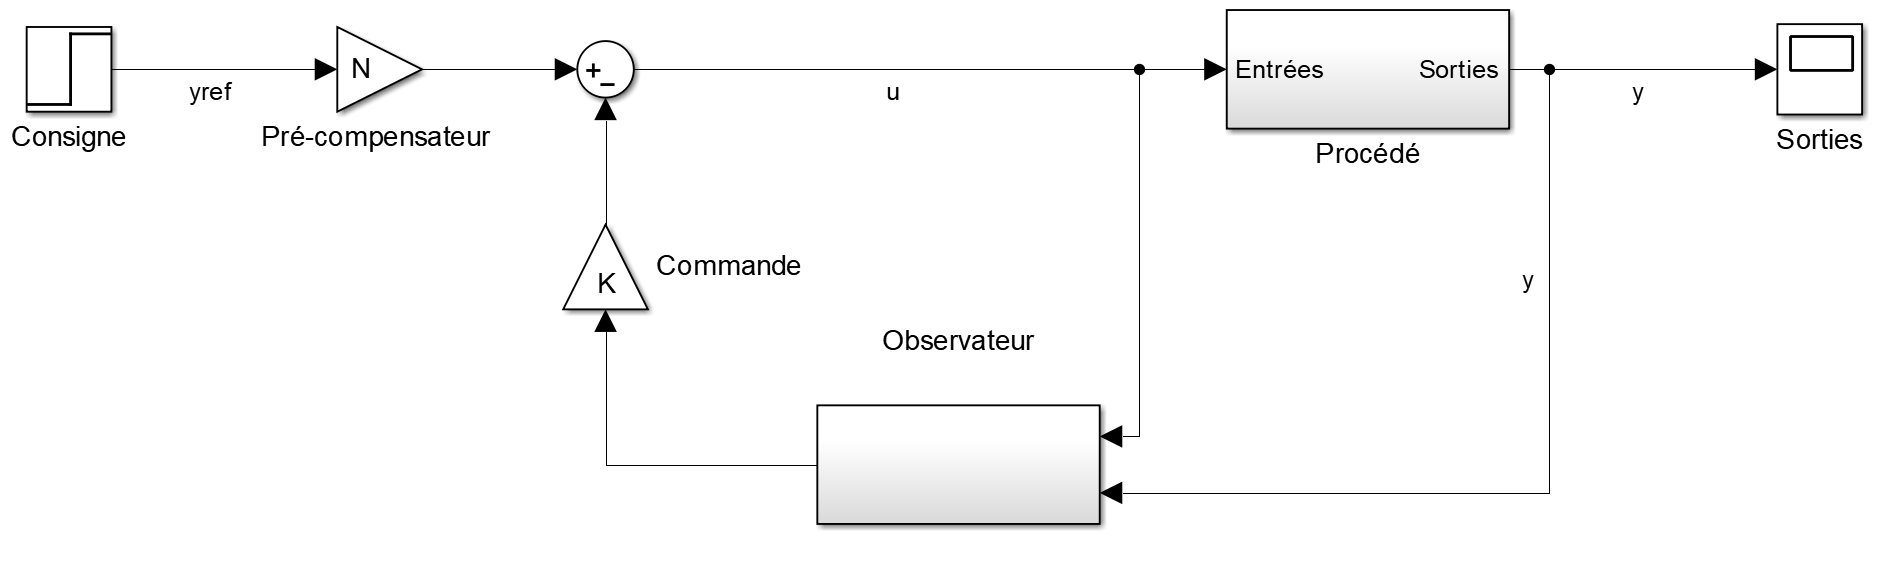
\includegraphics[width=.8\textwidth]{./page_de_garde/schemaRE.png}~\\[1cm]

\vfill
% logo fsi & eea
\begin{tabular}{cc}
   
\includegraphics[height=2cm]{./page_de_garde/logo_fsi.png} \hspace{2cm} &
    \hspace{2cm}
   
\includegraphics[height=2cm]{./page_de_garde/logo_eea.jpg} \\
\end{tabular}

% Bottom of the page
{\large \today}

\end{center}
\end{titlepage}
	

%page blanche
\newpage
~
\tableofcontents
\thispagestyle{empty}
\setcounter{page}{0}
%ne pas numéroter le sommaire


%espacement entre les lignes d'un tableau
\renewcommand{\arraystretch}{1.5}

%====================== INCLUSION DES PARTIES ======================
%
%~
\thispagestyle{empty}
%recommencer la numérotation des pages à "1"
\setcounter{page}{0}

\chapter*{Introduction}
\addcontentsline{toc}{chapter}{Introduction}
\label{chap:Intro}
% \begin{LARGE}
% Le rapport final inclura une hiérarchisation des émulations et des validations expérimentales, des justifications pour les choix matériels et logiciels, la prise en compte des informations à traiter sur une chaîne d'acquisition, un raisonnement construit pour les protocoles expérimentaux, un bilan sur le projet.\\
% A RÉÉCRIRE.
% \end{LARGE}
% Plan \\
% intro a refaire\\
% Les 2 chapitres de théories\\
% 1. Validation de la commande TC sur modèle NL \\
% 	1.1. Protocoles MIL/SIL\\
% 		1.1.1. MIL\\
% 		1.1.2. SIL\\	
% 	1.2. Commande temps continue\\
% 		1.2.1 Simulation \\
% 			1.2.1.1. Adaptation modèle (avec nl)\\
% 			1.2.1.2. Simulation et étude de perf\\
% 			1.2.1.3. Conclusion et Validation\\
% 		1.2.1 Sur moteur Réel (proto rapide)\\
% 			1.2.1.1. Adaptation modèle (avec nl)\\
% 			1.2.1.2. test et étude de perf\\
% 			1.2.1.3. Conclusion et Validation\\
% 2. Commande temps discret \\
% 	2.1. Contraintes hardware \\
% 		2.1.1. CAN / CNA (protocole correction, temps conversion, échantillonnage bits )\\
% 		2.1.2. C167 (ordo,taches,validation TR,temps calcul, fréquence fonctionnement)\\
% 		2.2.3. Conclusion  (contraintes tempo, squelette code correcteur)\\
% 	2.2. Transformation commande en TD\\
% 		2.1.1. Fonctions de transferts (observateur + retour état = 2 ft)\\
% 		2.1.2. Transformée en z\\		
% %	2.3. I et étude de perf\\
% %		2.3.1. Création commande TD matlab\\
% %		2.3.2. Simulation et étude de perf\\
% %		1.3.3. Conclusion et Validation\\
% 3. Implémentation \\
% 	3.1. Correction CAN/CNA\\
% 		3.1.1. Implémentation prog récupération lu/écrite\\
% 		3.1.2. Correction \\
% 		3.1.3. Validation \\
% 	3.2. Implémentation \\
% 		3.2.1. Description taches\\
% 		3.2.2. implémentation\\
% 	3.3. Validation et correction 

% 4. Bilan 
Pour l'UE \emph{Conception et mise en œuvre de Commande à temps réel}, nous devons réaliser la commande d’un système temps réel, à partir de la modélisation du procédé jusqu'à l'implémentation sur un micro-contrôleur. 

Notre problématique est la suivante : asservir un banc de moteurs à courant continu via un micro-contrôleur C167. Pour y parvenir, nous allons utiliser des références du Master EEA ISTR, 1er et 2ème année, ainsi que des ressources matérielles et logicielle disponibles dans les salles de TP de l'université. L'objectif de ce rapport est de vous présenter l'ensemble de nos travaux pour répondre à cette problématique. Ceux-ci ont été séparé en deux parties qui vous sont présentés ci dessous.

\paragraph*{Première partie}
La première partie de ce rapport contient toute la partie théorique. Celle-ci est décomposée dans les trois premiers chapitres dont nous faisons la liste ci dessous.

Le \emph{chapitre \ref{chap:modelisation} : Modélisation} contient l'étude physique qui nous a été donné en cours, le modèle le plus précis, non linéaire et variant, les différentes simplifications de celui-ci. 

Ensuite, dans le \emph{chapitre \ref{chap:analyse} : Analyse}, nous avons effectué une analyse de nos différents modèles afin de maîtriser l’impact de nos simplifications, étudier les performances de notre systèmes et définir celles souhaitées. Nous avons réalisé cela grâce, autant que nous avons pu, a une approche théorique et grâce à des simulations.

Le \emph{chapitre \ref{chap:commande} : Synthèse de commande}, qui est le dernier chapitre de la partie théorique, contient la conception de l'asservissement et l'étude des performances de celle-ci sur les différents modèles de notre système.

\paragraph*{Seconde partie}
Pour cette seconde partie, nous allons nous intéresser à l'implémentation de la commande. Nous serons dans un cadre de conception et validation de prototype à l'aide de protocole.

Le \emph{chapitre \ref{chap:Validation} Validation de la commande en temps continue sur le modèle non linéaire} va permettre d'introduire les protocoles utilisés pour valider les prototype de commande. Nous verrons si, au bout de ces test, nous devons oui ou non créer d'autres prototypes pour permettre la commande du système.

Dans le \emph{chapitre \ref{chap:commandeTempsDiscret} Commande à temps discret}, nous étudierons les moyens à notre disposition pour rendre la commande à temps discret.

Enfin, le \emph{chapitre \ref{:chap:Implementation}, Implémentation} portera sur la programmation de la loi de commande sur le C167. Nous devons alors pour cela, relever les problématiques liés à l’électronique et l'informatique.


% Dans le \emph{chapitre \ref{chap:suite} : Planification de la suite de l'asservissement }, nous détaillons comment nous allons testé la validité de nos modèles par rapport au modèle physique et les différentes étapes de la mise en \oe uvre sur micro-contrôleur. Ce chapitre nous permettra d'organiser au mieux notre démarche afin que la commande implémentée respecte bien les contraintes temps réel, garantisse la stabilité et les performances attendues tout en étant adaptée au support d'implémentation et au moteur asservi.

 % from sillabus :  les étudiants apprendront à réaliser la commande d’un système temps réel de bout en bout, du prototypage à la mise en œuvre sur un calculateur numérique (type microcontrôleur). Pour cela, ils apprendront à tenir compte des contraintes matérielles de la chaîne de contrôle-commande (i.e. du calculateur au procédé) pour effectuer le bon choix des différentes interfaces et de la meilleure architecture logicielle.	% Importation de introduction.tex

\chapter{Modélisation}
\label{chap:modelisation}

\section{Choix du formalisme et de la modélisation}
Notre modélisation sera basée sur les modèles physiques qui décrivent les différents constituants de notre système de procédé : deux moteurs couplés l'un à l'autre par un arbre simple. L'un étant générateur de force mécanique et l'autre générateur de courant afin de faire office de charge (il dissipe son énergie sur une résistance). Il y a aussi un tachymètre couplé à l'arbre principal par un réducteur.
Nos modèles seront donc des modèles de connaissances.

Nous avons choisis de faire une modélisation espace d'état pour différentes raisons. La première est que cette représentation permet d'étudier facilement la valeur des différents états (l'étude de la stabilité asymptotique, par exemple, en est simplifiée dans un modèle espace d'état). Elle permet aussi de garder les états non observables et non commandables dans le modèle, une modélisation par fonctions de transferts ne le permet pas. Ce choix nous permet aussi, pour la suite, de concevoir un asservissement par retour d'état basé observateur, qui est l'asservissement que nous avons choisis. Le choix d'un modèle de connaissance améliore aussi l'analyse de l'influence des différents paramètres du modèle, ce qui nous permettra d'affiner notre modèle lors des tests sur le système réel. 



\section{Maquette et équations physiques}
\subsection{Maquette :}
Voici, figure \ref{fig:schema0}, un schéma électrique et physique du banc qui fait office de procédé dans notre asservissement.
\begin{figure}[!ht]
\centering
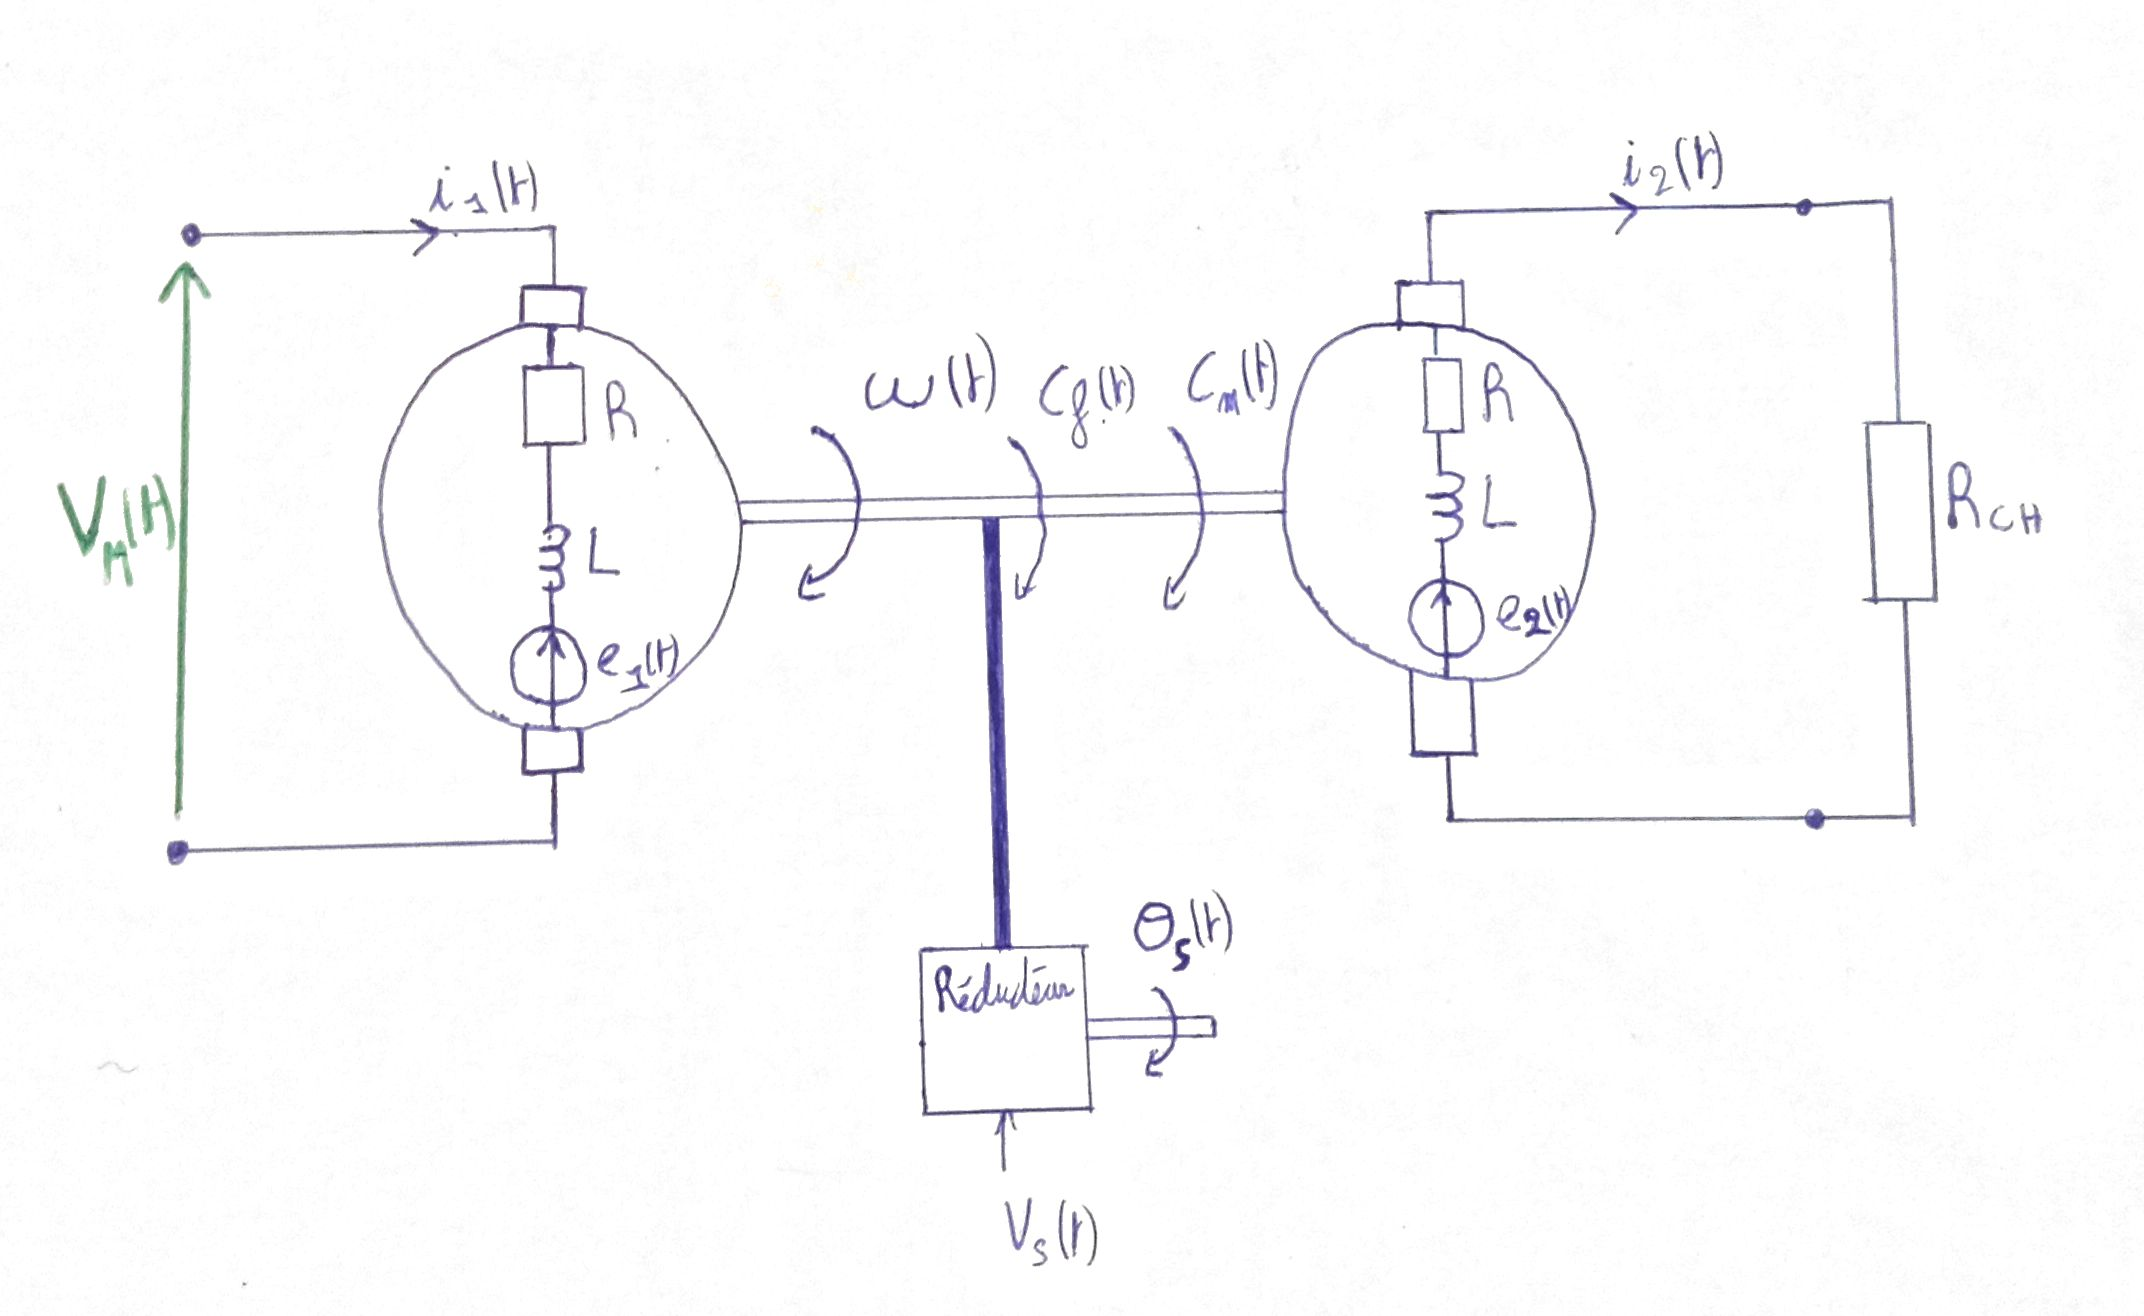
\includegraphics[width=.8\textwidth]{./I/images/schema0.png}
\caption{\label{fig:schema0}Schéma électrique/physique du banc moteur}
\end{figure}
Le circuit électrique de gauche correspond au Moteur à Courant Continue 1 (MCC) qui délivre la puissance mécanique à partir d'une tension d'entrée $V_M$. Celle-ci est l'entrée de notre procédé. Le schéma électrique de droite représente le MCC 2, générateur de puissance électrique qui fait office de charge en alimentant une résistance $R_{CH}$. Entre ces deux schémas électriques, se trouve une représentation de l'arbre, des forces qu'il subit, du réducteur et du tachymètre qui délivre une tension proportionnelle à la position du moteur, c'est le signal $V_s$, nous l'étudierons en tant que sortie. 

\subsection{Équations physique}\label{sub:equationPhysique}
Voici les différentes équations décrivant notre procédé:\\
\noindent\hspace{3mm}\textbullet  \hspace{1mm} Équations des moteurs :
\begin{eqnarray}
V_m(t)  					&=& 	R i_1(t) + L \frac{d   i_1(t)}{d t} + e_1(t) \\
e_2(t) 						&=& 	(R+R_{CH}) i_2(t) + L \frac{d i_2(t)}{d t}
\end{eqnarray}

\noindent\hspace{3mm}\textbullet  \hspace{1mm} Équations banc :
\begin{eqnarray}
J_2 \frac{d \omega(t)}{dt}   &=&    C_m(t) + C_f(t)    \\
 \frac{d \theta_s(t)}{dt}   &=&    \omega(t) \\
 e_1(t) &=& K_e \omega(t)\\
 e_2(t) &=& K_e \omega(t)\\
 C_m(t) &=& K_c i_1(t)-K_c i_2(t)\\
 C_f(t) &=& - \mu \omega(t)-C_0(t)\\
\label{eq:Rch} R_{CH}(t) &=& R_{CHn} + rR_{CH}(t) \Delta_1\\
\label{eq:nlC0} C_0(t) &=& -sign(C_m(t)C\\
 V_s(t)	&=& K_r K_s \theta_s(t)\\
 V_g(t) &=& K_g \omega(t)
\end{eqnarray}
O\`u :
\begin{description}
\item[$R$] La résistance de l'induit aux moteurs.
\item[$L$] L'inductance de l'induite des moteurs.
\item[$i_1(t),i_2(t)$] Respectivement le courant dans les moteurs 1 et 2.
\item[$e_1(t),e_2(t)$] Respectivement la force électromotrice des moteurs 1 et 2.
\item[$R_{CH}(t)$] Résistance de charge.
\item[ $J_2$ ] Inertie totale (somme des inerties du rotor, du réducteur et de la charge).
\item[$\omega_s(t)$] Vitesse radiale de l'arbre.
\item[$\theta_s$] Position de rotation de l'arbre.
\item[$C_m(t)$] Couple de l'arbre.
\item[$C_f(t)$]  Couple de frottement.
\item[$K_e$] Constante de force électromagnétique.
\item[$K_c$] Constante de couple.
\item[$\mu$] Coefficient de frottement visqueux.
\item[$C_0(t)$] Couple de frottement sec si rotation.
\item[$R_{CHn}$] Résistance de charge nominale.
\item[$rR_{CH}$] Rayon de l'incertitude de la résistance de charge.
\item[$\Delta_1$] Perturbation de la résistance de charge bornée en $[-1 ; 1]$.
\item[$K_r$] Facteur de réduction.
\item[$K_s$] Constante du potentiomètre.
\item[$K_g$] Constante de la génératrice tachymétrique.
\item[$V_g(t)$] Tension reflétant la vitesse de rotation de l'arbre. Sortie de performance non mesurée. 
\item[$C$] Couple de frottement sec si $\omega(t)$ assez grande.%
%\item[$ $] 
\end{description}

\subsection{Linéarisation}\label{sub:linearisation}
Les équations ci-dessous permettent de former un modèle du procédé. Néanmoins, l'équation \ref{eq:nlC0} exprime une non linéarité sur les frottements secs du banc moteur. Afin d'avoir un modèle linéaire du moteur, nous avons transformé cette non linéarité en incertitude.
Ainsi nous exprimons : 
\begin{eqnarray}
\label{eq:C0} C_0(t) &=& C_{0n} + rC_0 \Delta_2
\end{eqnarray}
O\`u : 
\begin{description}
\item[$C_{0n}$] Couple de frottement sec nominal.
\item[$rR_{CH}$] Rayon d'incertitude du couple de frottement sec.
\item[$\Delta_1$] Perturbation du couple de frottement sec bornée en $[-1 ; 1]$.
\end{description}
Nous avons maintenant des équations linéaires mais deux équations présentent des incertitudes dues aux perturbations $\Delta_1$ et $ \Delta_2$ respectivement liés à la température de la résistance de charge et à la non linéarité du couple de frottement sec.
\subsection{Invariance}\label{sub:invariance}
Nous souhaitons exprimer le modèle du procédé sous la forme d'un espace d'état linéaire et invariant, donc il faut rendre invariant nos équations. Pour cela, nous allons considérer que la résistance de charge $R_{CH}(t)$, exprimée dans l'équation \ref{eq:Rch} et $C_0(t)$, dans l'équation \ref{eq:C0} valent leurs valeurs nominales. 
\begin{eqnarray}
R_{CH}(t) &=& R_{CHn} \\
C_0(t)    &=& C_{0n}
\end{eqnarray}
Nous pouvons maintenant former un modèle linéaire et invariant.
\section{Modèle de niveau 0, modèle EE0}
Notre modèle présente 4 dynamiques, nous avons donc 4 états dans notre vecteur d'état.\\

Le vecteur d'état choisit est :
\begin{equation}
x(t)=\begin{bmatrix}
i_1\\
i_2\\
\Omega_m\\
\Theta_m\\
\end{bmatrix}
\end{equation} 
L'entrée $u(t)$ du modèle est $u(t)=V_m(t)$.\\

\noindent Les sorties sont $y(t)= \begin{bmatrix}
V_g(t)\\
V_s(t)
\end{bmatrix}$.\\

\noindent Le modèle d'ordre 4 vaut donc :
\begin{align}
\label{EE0}
\left\lbrace
\begin{aligned}
&\dot{x}(t) = \begin{pmatrix}
-\frac{R}{L}	& 	    0				& 0 &   -\frac{K_e}{L}	\\
      0			&  -\frac{(R+R_{ch})}{L}&0	&	-\frac{K_e}{L}	\\
0&	0&	0 & 1\\
\frac{K_c}{J_2}	&	\frac{K_c}{J_2}		&0&	\frac{\mu}{J_2}
\end{pmatrix}x(t)+\begin{pmatrix}
\frac{1}{L}\\0\\0\\0
\end{pmatrix}u(t)\\
&y(t) = \begin{pmatrix}
0&	0&	0 & K_g	\\
0&	0&	K_rK_s	&	0\\
\end{pmatrix}x(t)
\end{aligned}
\right.
\end{align}
\section{Espace d'état d'ordre 3, modèle EE1}
Afin de facilité la création d'une commande, nous avons retiré l'état $i_2(t)$ de l'état de la modélisation. Il permettra une validation intermédiaire. \\

\noindent L'état vaut maintenant \begin{equation}
x(t)=\begin{bmatrix}
i_1\\
\Omega_m\\
\Theta_m\\
\end{bmatrix}
\end{equation} 
\noindent L'entrée et les sorties n'ont pas changées. \\

\noindent L'espace d'état, d'ordre 3, vaut : 
\begin{align}
\label{EE0}
\left\lbrace
\begin{aligned}
&\dot{x}(t) = \begin{pmatrix}
-\frac{R}{L}	& 	     0 &   -\frac{K_e}{L}	\\
0&	0 & 1\\
\frac{K_c}{J_2}	&	0&	\frac{\mu}{J_2}
\end{pmatrix}x(t)+\begin{pmatrix}
\frac{1}{L}\\0\\0
\end{pmatrix}u(t)\\
&y(t) = \begin{pmatrix}
0&		0 & K_g	\\
0&		K_rK_s	&	0\\
\end{pmatrix}x(t)
\end{aligned}
\right.
\end{align}
\section{Espace d'état d'ordre 2, modèle EE2}
Pour correspondre avec un modèle de comportement, nous allons à nouveau réduire la représentation d'état ~\eqref{EE0} pour obtenir un modèle d'ordre 2. Pour cela, nous allons annuler l'effet des dynamiques des courants $i_1$ et $i_2$ qui sont beaucoup plus grandes que les dynamiques de $\omega$ et $\theta$, qui sont celles que nous sommes capable de mesurer et que nous souhaitons asservir. Ainsi nous avons un espace d'état o\`u il sera plus facile de concevoir un retour d'état. Le système d'ordre 3 servira donc de modèle permettant une validation intermédiaire entre celui d'ordre 2 et celui d'ordre 4.\\

\noindent Le vecteur d'état vaut maintenant : \begin{equation}
x(t)=\begin{bmatrix}
\Omega_m\\
\Theta_m\\
\end{bmatrix}
\end{equation}

\noindent Le modèle espace d'état d'ordre 2 vaut :\\

\begin{align}
\label{EE2}
\left\lbrace
\begin{aligned}
&\dot{X}(t) 
=
 \begin{pmatrix}
0 &	1 \\
0	&	-\frac{(K_c K_e)}{J_2 R}-\frac{\mu}{J_2}\\
\end{pmatrix}X(t)
+
\begin{pmatrix}
\frac{K_c}{J_2 R}\\
0
\end{pmatrix} 
V_m(t)\\
&Y(t) = \begin{pmatrix}
0	&	K_g	\\
K_rK_s	&	0	\\
\end{pmatrix}X(t)
\end{aligned}
\right.
\end{align}



\chapter{Analyse}
\label{chap:analyse}
Dans ce chapitre, nous allons dans une première partie, étudier la stabilité de nos différentes modélisations (espace d'état d'ordre 4, 3 et 2), puis leurs commandabilités et observabilités. Dans une seconde partie, nous étudierons les performances dynamiques des différents modèles à travers une analyse temporelles et fréquentielle. Dans l'ensemble du chapitre sera abordé l'impact des simplifications effectués sur les modèles espace d'état d'ordre 3 et 2.
Comme nous souhaitons asservir le procédé en vitesse et non en position, nous étudierons la sortie de performance $V_g(t)$ des modèles  et non $V_s(t)$. 

\section{Analyse des modèles}
\subsection{Stabilité}
Nous avons décidé d'étudier la stabilité asymptotique afin de savoir si l'ensemble des états de nos modèles sont stables et non uniquement ceux qui sont observables comme en stabilité BIBO. \\

\noindent Les valeurs propres de notre système d'ordre 4 sont : (calculé à l'aide de matlab)\\
\begin{equation}
{0 ; -132749,8861 ; -4,0655 ; -7748,0483 }
\end{equation}
Nous remarquons que les valeurs propres sont toutes à partie réelle négatives, le système d'ordre 4 est donc asymptotiquement stable.

\noindent Les valeurs propres de notre système d'ordre 3 sont : (calculé à l'aide de matlab)\\
\begin{equation}
{ 0 ; -7748,0484 ; -3,9516 }
\end{equation}
Nous remarquons que les valeurs propres sont toutes à parties réelles négatives, le système d'ordre 3 est donc asymptotiquement stable.\\

C'était prévisible car le modèle d'ordre 3 est une simplification du modèle d'ordre 4, qui est stable. Nous remarquons aussi que la troisième valeur propre du système d'ordre 3, qui normalement doit être similaire à la troisième valeur propre du système d'ordre 4 a légèrement variée. Cette différence est une première conséquence de la perte d'une dynamique engendrée par la simplification.

\noindent Les valeurs propres de notre système d'ordre 2 sont : (calculé à l'aide de matlab)\\
\begin{equation}
{0 ; -3,9506 }
\end{equation}
Nous remarquons que les valeurs propres sont toutes à parties réelles négatives, le système d'ordre 2 est donc asymptotiquement stable.\\
Comme précédemment, cette conclusion était prévisible, néanmoins on remarque une autre conséquence de la simplification sur la seconde valeur propre qui est légèrement différente de celle du modèle d'ordre 3.

\subsection{Commandabilité}
L'étude de la commandabilité d'un système nous permettra de savoir quels états sont commandables, c'est à dire qu'il sera possible de modifier la dynamique qu'ils représentent par un asservissement. Cette étude se fera uniquement sur l'espace d'état d'ordre 4 car les deux autres modèles découlent de celui-ci. Un système (sous forme d'espace d'état) est commandable, d'après le critère de Kalman, si 
la matrice de commandabilité $\mathcal{C}_m$ est de rang plein donc égale à la dimension de A.\\

Où, $ \mathcal{C}_m = \begin{bmatrix} B  & AB & \dots & A^{n−1}B\end{bmatrix}$
Nous avons étudié la commandabilité sur matlab et le résultat est que :
$$rang(\mathcal{C}_m) = n = 4 $$
Donc le système est commandable. Cela nous permet de mettre en place un retour d'état. 

\subsection{Observabilité}
L'étude de l'observabilité d'un système nous permettra de savoir quels états sont observables, c'est à dire s'il est possible de déterminer la valeur des états à partir de mesures de la sortie. Cette étude se fera uniquement sur l'espace d'état d'ordre 4 car les deux autres modèles découlent de celui-ci. Un système (sous forme d'espace d'état) est observable, d'après le critère de Kalman, si 
la matrice d'observabilité  $\mathcal{O}$ est de rang plein donc égale à la dimension de A.\\

Où, $ \mathcal{O} = \begin{bmatrix} C \\ CA \\ \vdots \\ CA^{n−1} \end{bmatrix}$
Nous avons étudié l'observabilité sur matlab et le résultat est que :
$$rang(\mathcal{O}) = dim(A)=4 $$
Donc le système est observable, néanmoins intuitivement ce résultat semble faux.

\section{Analyse temporelle et fréquentielle}
Nous avons étudié les performances de nos modèles grâce à deux types de réponses : 
\begin{itemize}
\item Une réponse à un échelon unité (voir figure \ref{fig:echelon}).
\item Une réponse fréquentielle représentée par un diagramme de Bode (voir figure \ref{fig:bode}).
\end{itemize}

\begin{figure}[!ht]
\centering
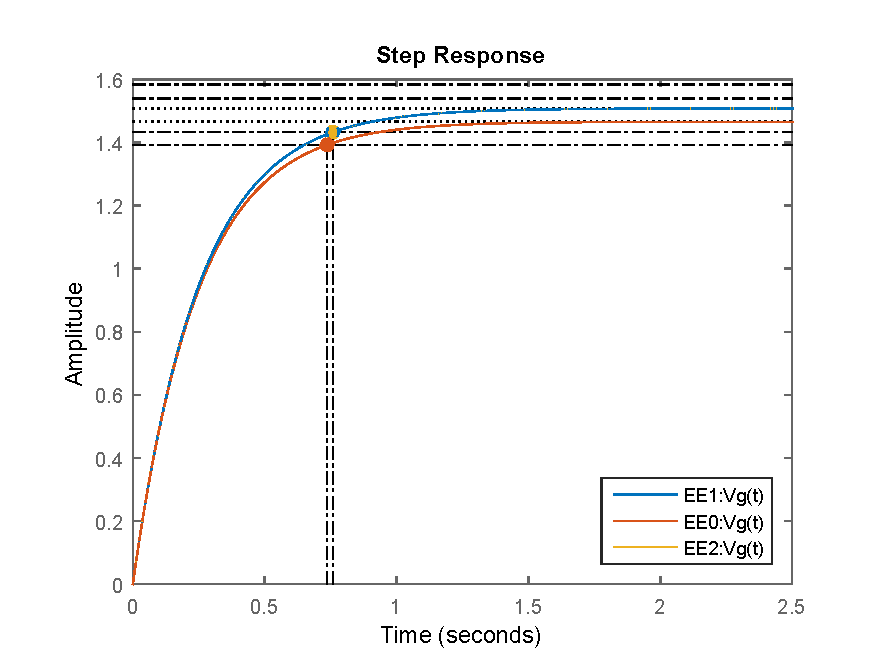
\includegraphics[width=.8\textwidth]{./II/images/echelon.pdf}
\caption{\label{fig:echelon}Réponse à un échelon unité de $V_g(t)$ des modèles EE0, EE1 et EE2.}
\end{figure}
\begin{figure}[!ht]
\centering
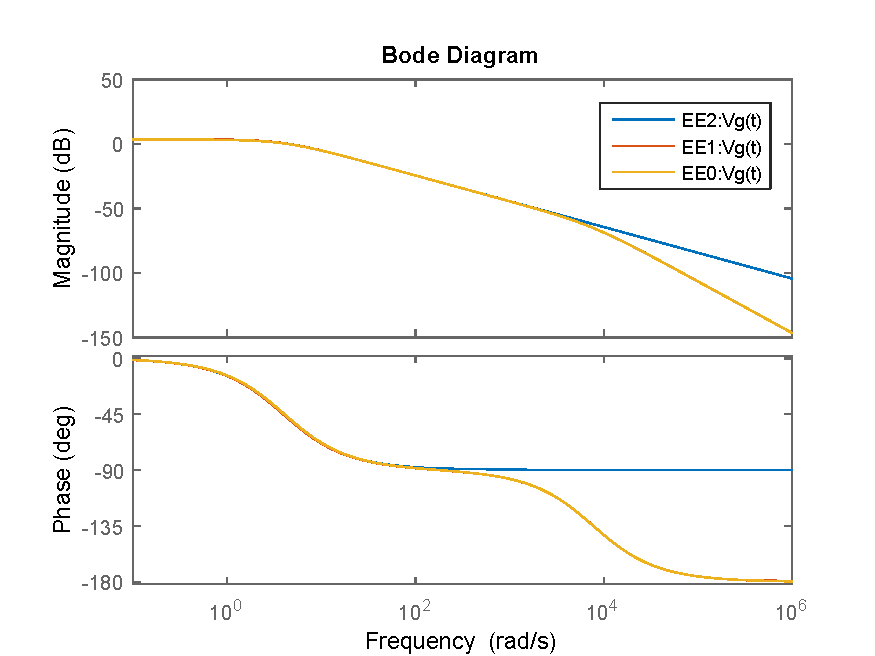
\includegraphics[width=.8\textwidth]{./II/images/bode.pdf}
\caption{\label{fig:bode}Diagramme de Bode sur $V_g(t)$ des modèles EE0, EE1 et EE2.}
\end{figure}

\subsection{Performances Statiques}
Nous étudions $V_g(t)$ en temps que sortie de performance (figure \ref{fig:echelon}).\\
Nos modèles présentent des gains statiques qui varient d'un modèle à l'autre, à cause des simplifications : \\

\noindent Gain statique de EE0 : $1,4658$\\

\noindent Gain statique de EE1 : $1.5080$\\

\noindent Gain statique de EE0 : $1.5080$\\

On peut constater qu'entre le modèle EE0 et le modèle EE1, il y a une erreur de $0.0423$ et qu'en le modèle EE1 et le modèle EE2 l'erreur vaut $2.0241*10^{-8}$. La première simplification engendre une erreur d'environ $2\%$ et la suivante de le l'ordre de $10^{-8}\%$. L'asservissement risquera donc de présenter une erreur statique causée par ces simplifications.

\subsection{Performances dynamiques}
Nous étudions $V_g(t)$ en temps que sortie de performance (figure \ref{fig:echelon}).\\
Nous avons choisis d'étudier le temps de montée, le temps de réponse et le dépassement car ce sont des paramètres précis et déterminants en terme de performances. 

\noindent Temps de montées :\\
\noindent Sur EE0 : 0.5404s \\
\noindent Sur EE1 : 0.5560s\\
\noindent Sur EE2 : 0.5561s\\
\noindent Erreur de EE0 à EE1 : 0.0156 s (2.8826$\%$)\\
\noindent Erreur de EE1 à EE2 : 1.3830e-04 s(0.0249$\%$)\\
Nous pouvons remarquer que le temps de montée est aux alentours d'une demie seconde. Les différences entre les temps de montées des différents modèles risquent de créer une erreur sur l'asservissement, en effet elle témoigne d'une différence dans les dynamiques des modèles (ce qui est une conséquence logique de la simplification). Le test de la commande sur EE0 risque de démontrer une erreur dynamique.\\

 
\noindent Temps de réponses à $5\%$ :\\
\noindent Sur EE0 : 0.7370 s\\
\noindent Sur EE1 : 0.7582 s\\
\noindent Sur EE2 : 0.7583 s\\
\noindent Erreur de EE0 à EE1 : 0.0212 s (2.8821$\%$)\\
\noindent Erreur de EE1 à EE2 : 5.9211e-05 s(7.8089e-05$\%$)\\
Comme pour la performance précédente , la valeur du temps de réponse varie et cela entrainera de potentielles erreurs d'asservissement.

\noindent Dépassements  :\\
Le modèle en boucle ouverte ne présente pas de dépassement.
\subsection{Analyse fréquentielle}
On peut remarquer sur le diagramme de Bode, figure \ref{fig:bode}, qu'il y a une compensation pôle zéro dans le modèle EE0 car nous avons uniquement trois changements d'allures. Cela se confirme sur une vue des pôles et des zéros sur un plan complexe (voir figure \ref{fig:poles}) ou une fonction de transfert. Cette figure met en évidence la compensation d'un pôle électrique qui agis à haute fréquence. Sur le diagramme de Bode, nous pouvons aussi constater que les modèles semblent avoir des réponses fréquentielles assez similaires. On peut aussi voir l'absence de la dernière dynamique de EE2 due à la simplification.

\begin{figure}[!ht]
\centering
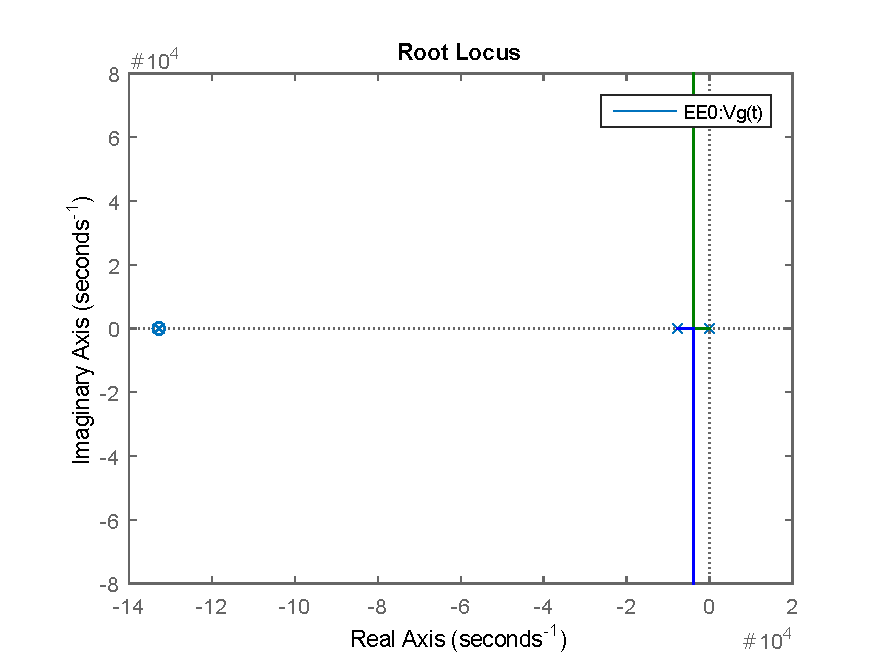
\includegraphics[width=.5\textwidth]{./II/images/poles.pdf}
\caption{\label{fig:poles}Pôles et zéros dans le plan complexe du transfert vers $V_g(t)$ du modèles EE0.}
\end{figure}

\chapter{Synthèse de commande}
\label{chap:commande}
\section{Commande du système d'ordre 2}
\subsection{Rédaction du cahier des charges et démarche de réponse}
Après l'étude que nous venons de réaliser sur notre système, nous allons ici exprimer les attentes que doit réaliser la commande que nous allons implémenter. Nous souhaitons avoir : \begin{itemize} 
\item Erreur de position nulle.
\item Pas d'oscillations
\item Temps de réponse inférieur à 1 seconde.
\end{itemize}
La commande de notre système doit permettre d'asservir le système en vitesse, par rapport à une consigne. Pour respecter, nous allons réaliser un placement de valeurs propres par retour d'état.



\subsection{Calcul du retour d'état}
\label{sub:Calcul du retour etat}
Pour garantir les performances dynamiques souhaitées, nous allons appliquer un placement de pôles par retour d'état. Ce réajustement des valeurs propres de la matrice dynamique du système nous permettra de répondre aux attentes du cahier des charges si le choix de celles-ci est correct. De même, nous devons choisir des valeurs propres qui ne sont pas être trop éloignées de celles du procédé, pour ne pas être trop exigeant avec la commande et le système. Nous avons avec ces spécifications choisi les valeur propres suivantes :
\begin{equation}
\label{equation:valeurPropres}
\lambda = \begin{pmatrix}
-4 &-5
\end{pmatrix}
\end{equation}
La commande par retour d'état est une méthode d'asservissement qui permet d'effectuer un placement de pôles. Cette correction se réalise grâce à un gain $K$ qui va corriger l'état $x$ d'un système. Cette loi de commande s'écrit : 
\begin{equation}
u(t) = Ny_{ref}-Kx(t)
\end{equation} avec $N$ un gain de pré-compensation, $y_{ref}$ la vitesse de référence, $x(t)$ la sortie mesuré du système et $K$ le gain de retour. Si l'on applique cette loi à notre système en espace d'état, on obtient : 
\begin{align*}
\left\lbrace
\begin{aligned}
&\dot{X}(t) = (A-BK)X(t) + BNy_{ref}\\
&Y = CX(t)
\end{aligned}
\right.
\end{align*}
Ainsi la nouvelle dynamique du système est donnée par la matrice $A' = (A-BK)$ et doit admettre les valeurs propres que nous désirons appliquer à notre système. $A$ et $B$ étant des paramètres du système, nous allons utiliser le gain $K$ pour répondre à ce problème. Avec la fonction $place$ de MATLAB, nous sommes capable de concevoir ce vecteur $K$. 


\subsection{Observateur ordre plein sur modèle d'ordre 2\label{sub:constructionObeservateur}}
Pour pouvoir réaliser notre commande par retour d'état, nous devons tous d'abord reconstruire l'ensemble des états du système dont nous n'avons pas accès. Dans notre cas, nous disposons d'une mesure de la position du moteur $\theta$ avec $V_s$ mais aucune mesure nécessaire pour au minimum reconstruire cet état.


Nous préférons reconstruire les deux états $\Omega$ et $\theta$ à partir de $V_s$ et de l'entrée du modèle d'ordre 2 pour simplifier les calculs nécessaire à sa construction. Les équations de l'observateur sont présentées par :
\begin{align*}
\left\lbrace
\begin{aligned}
&\dot z (t) = Fz(t) + Gy(t) + Hu(t)\\
&\hat x (t)= Mz(t) + Ny(t)\\
&\epsilon (t)= x-\hat{x}
\end{aligned}
\right.
\end{align*}
 où $x$ représente l'état du système, $\hat{x}$ l'état du système reconstruit et $\epsilon$ l'erreur d'estimation à un temps $t$. Nous souhaitons contrôler la dynamique de ce paramètres pour pouvoir estimer correctement notre système. Pour cela, nous nous interressons à : 
\begin{eqnarray}
&&\dot{\epsilon} = \dot{x} - \dot{\hat{x}}\\
\label{equ:obs2}&\Leftrightarrow & \dot{\epsilon} = Ax +Bu - F\hat{x} - Gy - Hu \text{   en considérant }M=1 \text{ et } N = 0\\
& \Leftrightarrow & \dot{\epsilon} = Ax - F\hat{x} - GCx + u(B-H)\\
& \Leftrightarrow & \dot{\epsilon} = (A-GC-F)x + F\epsilon + u(B-H)
\end{eqnarray}
Il vient alors $F = A-GC$ et $B=H$ pour obtenir $\dot{\epsilon} = F\epsilon$. Ainsi l'erreur d'estimation est autonome et ne dépend pas des entrées et sorties du système, et il vient $\epsilon(t) = e^{Ft}\epsilon(0)$. Les valeurs propres de $F$ vont ainsi déterminer la dynamique de l'erreur d'estimation, nous choisissons de les faire dépendre des valeurs propres désirées dans la partie \ref{sub:Calcul du retour etat} en les multipliant par 3, pour une convergence encore plus rapide. 
\begin{equation}\label{eqn:vpObservateur}
v_{p_{obs}} = 3\times \lambda
\end{equation}

\subsection{Construction de l'asservissement}
Maintenant que l'observateur et le gain du retour d'état sont construits, nous allons les réunir pour former un unique modèle de commande. Pour ce modèle du système bouclé, nous prenons comme vecteur d'état $X=\begin{pmatrix}
X&\epsilon
\end{pmatrix}^T$ et nous obtenons par construction :
\begin{align*}
\label{eqn:systemeEE2_bf}
\left\lbrace
\begin{aligned}
& \dot{X} = \begin{pmatrix}
(A-BK) & -BK\\
0& F
\end{pmatrix}X+\begin{pmatrix}
BN\\0
\end{pmatrix}y_{ref} \\
& y(t) = \begin{pmatrix}
C & 0
\end{pmatrix}X
\end{aligned}
\right.
\end{align*} 

Le gain de pré-compensation $N$ est à partir gain statique du transfert entre $Vg$ et $y_{ref}$ noté $G_{Vg/y_{ref}}$ pour permettre une erreur de position nulle. Il est : 
\begin{equation}
N = \frac{1}{G_{Vg/y_{ref}}}
\end{equation}


Cependant, pour permettre un asservissement du système en vitesse $\omega$, nous devons modifier légèrement le résultat obtenu. La description telle qu'elle est donnée de ce système bouclé va asservir le système en position, à cause du changement de dynamiques de la position $\theta$ avec le retour d'état. Pour prévenir à cette mauvaise commande, nous avons annulé le retour de la mesure de position dans le système bouclé. 


A partir de ce modèle, nous allons être capable d'éprouver la commande obtenu de manière théorique et avec une simulation SIMULINK.

\section{Validation de la commande}
\subsection{Validation théorique}
Pour commencer, nous allons identifier les valeurs propres de notre système \ref{eqn:systemeEE2_bf} afin de de connaitre les effets de l'observateur sur le retour d'état, même si a priori celui ci est autonome. Nous obtenons les $\lambda_i$ valeurs propres suivantes : $-5$, $-4$, $-15$ et $-12$. Nous remarquons que les $\lambda_i$ n'ont pas été modifiées : nous avons les valeurs propres désirées par la commande et nous avons celles désirées pour l'erreur d'estimation de l'observateur. 

\subsection{Simulation SIMULINK}
Pour compléter la validation de la commande, nous avons crée un prototype avec SIMULINK pour pouvoir simuler une réponse temporelle de la commande de notre système. La description du fichier se trouve en annexe \ref{Annex:SIMULINK_RE}. Nous observons sur les figures suivantes la réponse temporelle à une référence $y_{ref} = 1$ : 
\begin{figure}[!ht]
\begin{center}
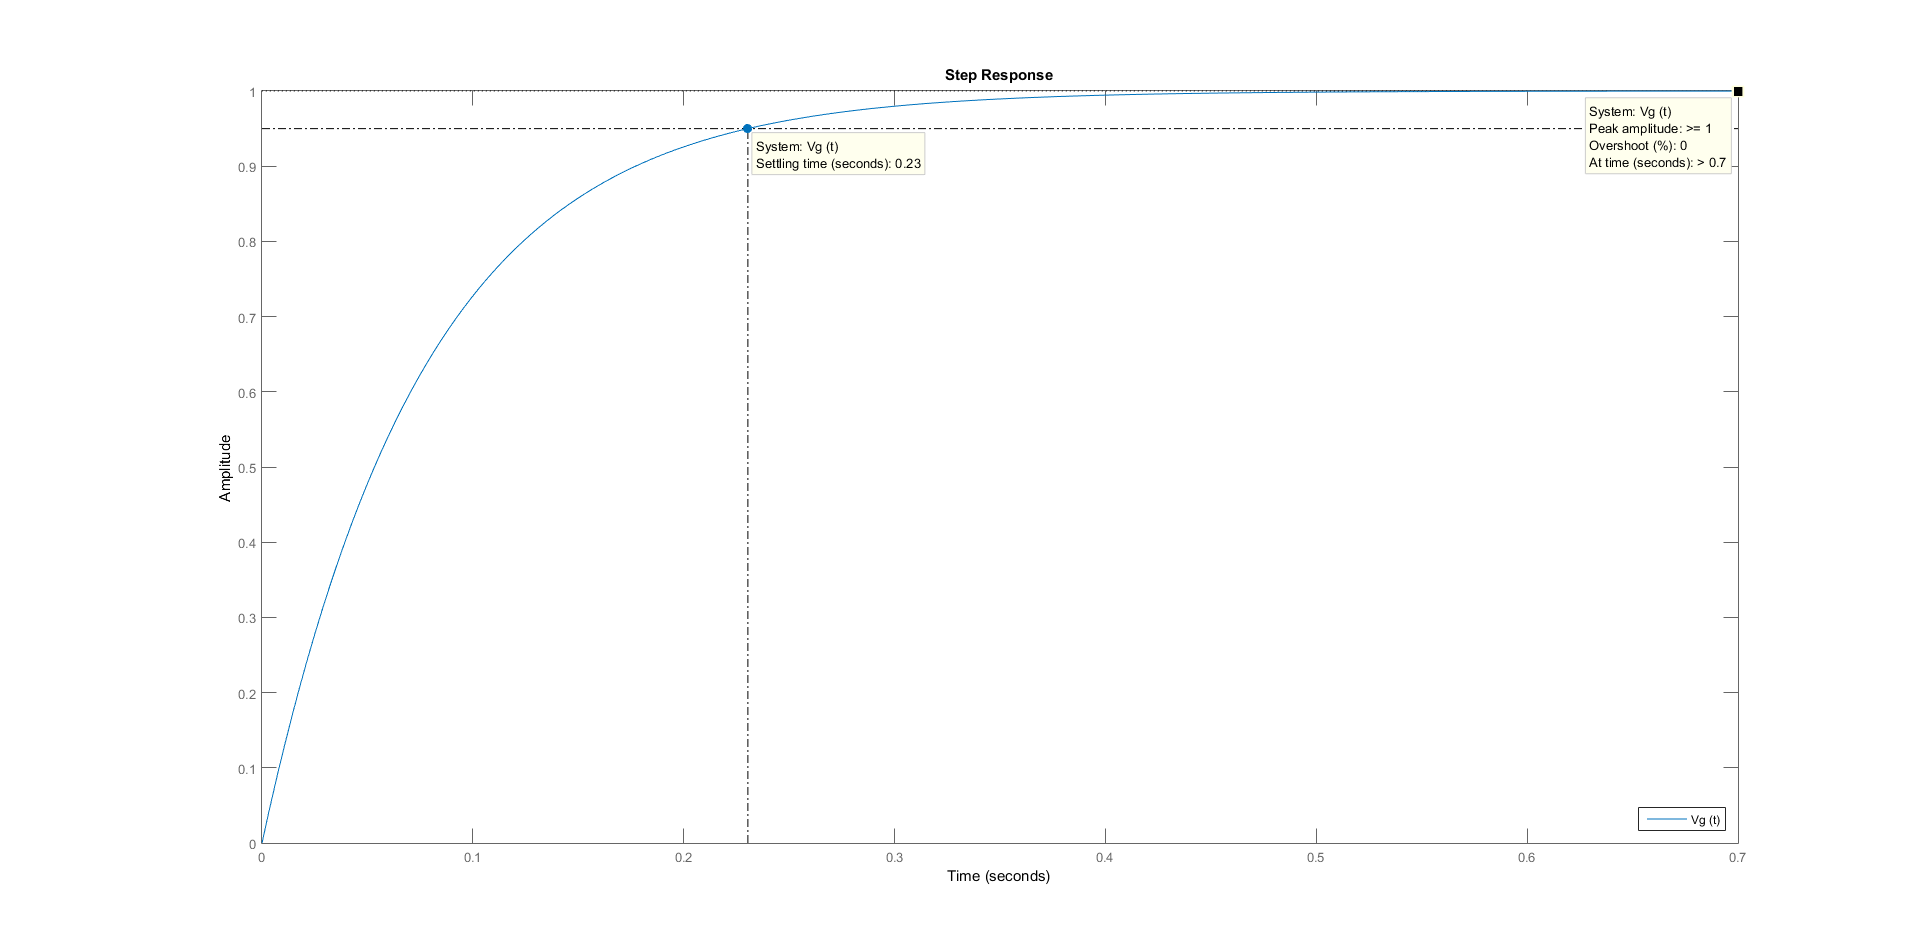
\includegraphics[width = \textwidth]{./III/figure/stepEE2bf.png}
\caption{Réponse du système asservi}
\end{center}
\end{figure}
La réponse du système $Vs$ simulé correspond aux changement de dynamique que nous avons espéré. De plus, après une observation de la commande $u(t)$ appliquée sur le système, nous voyons que la tension maximale envoyée est borné dans l'ordre de grandeur des valeurs admises par le système physique. 


\subsection{Analyse boucle fermé du modèle d'ordre 3}
Notre commande respecte le cahier des charges, nous validons ainsi la commande pour notre modèle d'ordre 2. Nous allons maintenant valider cette même commande sur des modèles supérieur et plus complexes pour compléter sa validation. En effet, notre modèle a été très simplifié pour permettre la création du commande facilement. Si nous arrivons a prouvé que cette commande marche sur des systèmes plus complexes, alors nous aurons prouvé que les dynamiques que nous avons simplifiés ne vont pas perturbé notre commande.

\section{Validation sur les modèles d'ordre supérieur}
\subsection{Changement de base du modèle d'ordre 3}
Dans un premier temps, nous regarderons les effets de l'implantation de l'observateur d'ordre 2 sur les modèles d'ordre supérieur et plus précisément l'erreur d'estimation et le placement des valeurs propres, puis nous simulerons la commande obtenu pour observé les modifications des réponses.

Pour intégrer l'observateur dans un espace d'état d'ordre supérieur, nous avons du réorganiser les états du modèle, ici le modèle d'ordre 3, de façon à ce que les états reconstruits avec l'observateur soient en haut, $x_1$, et les non reconstruits en bas $x_2$.

\noindent\textbullet\hspace{2mm} États reconstruits : $\Omega_m$ et $ \Theta_m$.

\noindent\textbullet\hspace{2mm} États non reconstruits : $i_1$

On obtient le vecteur d'état suivant : 
\begin{equation}
\overline{X} = \begin{bmatrix}
\theta\\
\omega\\
i_1\\
\end{bmatrix} = \begin{pmatrix}
x_1\\x_2
\end{pmatrix}
\end{equation}
donc $x_1 = \begin{bmatrix}
\theta\\
\omega\\ \end{bmatrix}$ et $x_2 = i_1$. Pour passer de $X$ à $\overline{X}$, il faut utiliser une matrice de passage $P_X$ définit par :
 \begin{eqnarray}
 P_X &/&  \overline{X} =P_X \cdot X \\
 P_X &=&\begin{bmatrix}
 0 & 0 & 1 \\
 1 & 0 & 0 \\
 0 & 1 & 0 \\
\end{bmatrix}  \\
 \end{eqnarray}
Maintenant, nous devons calculer $\overline{A}$, $\overline{B}$, $\overline{C}$, $\overline{D}$ pour le nouvel espace d'état lié à $\overline{X}$.
\begin{equation}%
	\left\lbrace%
	\begin{matrix}
		\overline{A} &=& P^{-1} A P \\%
		\overline{B} &=& P^{-1} B \\%
		\overline{C} &=& C P%	
	\end{matrix}
\right.%
\end{equation}

\subsection{Analyse du changement de base et de l'erreur de reconstruction}
Maintenant que nous avons replacé le modèle d'état, nous pouvons commencer l'analyse de celui ci. Avec les résultats obtenus pendant les séances de TD et de cours, nous avons obtenu une relation de la dynamique de l'erreur \begin{equation}\label{eqn:erreurRecompoOrdreSup}
\dot{\epsilon} = F\epsilon - A_2x_2
\end{equation}
avec $A_2$ la partie de la matrice $A$ qui lie l'état $\dot{x_1}$ à $x_2$ dans la nouvelle base. Cet élément modifie les résultats que nous avons obtenu pour le modèle d'ordre 2 en indiquant que l'évolution de l'erreur de reconstruction des états n'est plus en fonction uniquement d'elle même, mais aussi des états qui n'ont pas été reconstruits. Cette nouvelle donné va perturbé la convergence de la reconstruction de l'erreur, nous n'arriverons pas à reconstruire l'ensemble des états. 


Nous allons étudier les nouvelles valeurs propres du système bouclé pour vérifier si celles si correspondent toujours au cahier des charges, en modélisant un espace d'état qui admet comme vecteur d'état $x=\begin{pmatrix}
\overline{X}&\epsilon \end{pmatrix}^T$. Nous obtenons : $-7748$, $-20.61$, $ -3.832 \pm 6.931$ et $-2.784$, la stabilité asymptotique en boucle fermé est toujours respectée.



Pour continuer l'analyse de cette commande, nous obtenons à partir de tracé \emph{MATLAB} les réponses temporelles du système en boucle fermé avec les caractéristiques suivantes : \begin{itemize}
\item Le gain statique n'est plus respecté. Nous commençons à voir apparaitre une erreur de position en régime statique. Cette erreur est due à l'erreur de reconstruction de 
\item le temps de réponse reste dans la clause du cahier des charges et pas d'oscillations
\end{itemize} 


Pour finir l'analyse de la boucle fermé, nous allons étudier le transfert de $V_g(t)$ avec la consigne et le comparer avec celui du modèle d'ordre 2. Nous obtenons le diagramme de Bode en figure \ref{fig:transfertX/consigne}.
\begin{figure}[!ht]
\centering
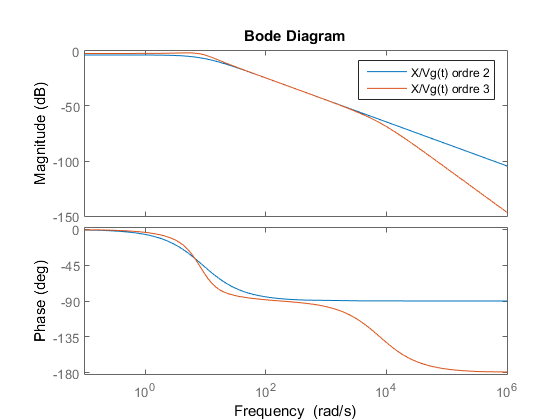
\includegraphics[width = .5\textwidth]{./III/figure/bode_Tpert_EE1.png}
\caption{Transfert de la boucle fermé, modèle linéaire d'ordre 3\label{fig:transfertX/consigne}}
\end{figure}


Le résultat que nous obtenons confirmes la stabilité asymptotique établie précédemment, cependant les différences notables avec le transfert du modèle d'ordre 2 en basse fréquence explique pourquoi nous n'avons pas pu respecter exactement le cahier des charges. 

\subsection{Changement de base du modèle d'ordre 4 et intégration de la commande\label{sub:observateurSurModelO4}}
De la même manière que pour le modèle d'ordre 3, nous effectuons un changement de base avec la matrice de passage : \begin{equation}
P = \begin{pmatrix}
0 &0& 1& 0\\ 0& 0& 0& 1\\1& 0& 0& 0\\ 0& 1& 0& 0
\end{pmatrix}
\end{equation}
Nous obtenons ainsi comme dans la section précédente, un modèle d'ordre 4 qui a comme vecteur d'état : 
\begin{equation}
\overline{X} = \begin{pmatrix}
\theta & \omega & i_1& i_2
\end{pmatrix}^T
\end{equation}

Les performances du système bouclé ont les mêmes problèmes que pour le modèle d'ordre 3. Les reconstructions des états ne convergent pas vers 0, comme nous l'avions vu précédemment, ce qui perturbe l'asservissement en vitesse.

De plus, les approximations de modélisation ont montré dans l'analyse des modèles une erreur statique que nous ne pouvons pas corriger avec une commande construite sur le modèle d'ordre 2. Nous avons toutefois voulu analyser le transfert entre $Vg$ et la consigne et obtenons :
\begin{figure}[ht]
\centering
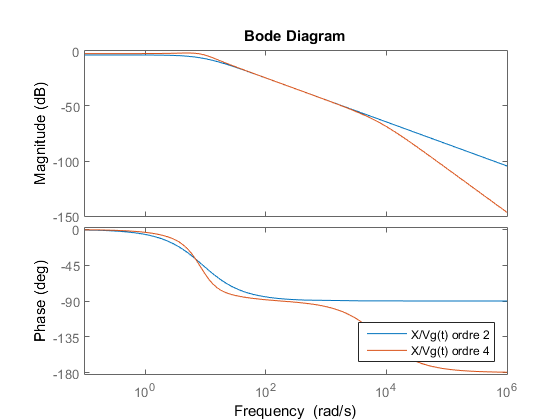
\includegraphics[width = .5\textwidth]{./III/figure/bode_Tpert_EE0.png}
\caption{Transfert de la boucle fermé, modèle linéaire d'ordre 4}
\end{figure}
Nous avons de plus amples écart en basse fréquence avec un dépassement encore plus grand que pour le modèle d'ordre 3. Ce dépassement joue beaucoup sur les oscillations du système en boucle fermé. Le cahier des charges n'est encore une fois pas respecté pour ce modèle mais admet un temps de réponse proche de celui du modèle d'ordre 2.

En sachant ceci, nous savons que les dynamiques qui ont été simplifiés ne sont pas l'origine des écarts que nous venons d'exposer, il s'agit de la dynamique de l'observateur qui n'est pas optimale. 

\subsection{Étude de la réponse entre l'erreur de reconstruction par rapport à une commande}\label{sub:etudeTransfertErreurCommande}
Avec les changements de base calculé précédemment, nous avons souhaité analysé les transferts entre l'erreur de reconstruction $\epsilon$ et la commande $u$. Pour cela, nous avons utilisé une réponse temporelle affichée en figure \ref{fig:repTemporelle_erreurReconstruction}.  
\begin{figure}[!ht]
\centering
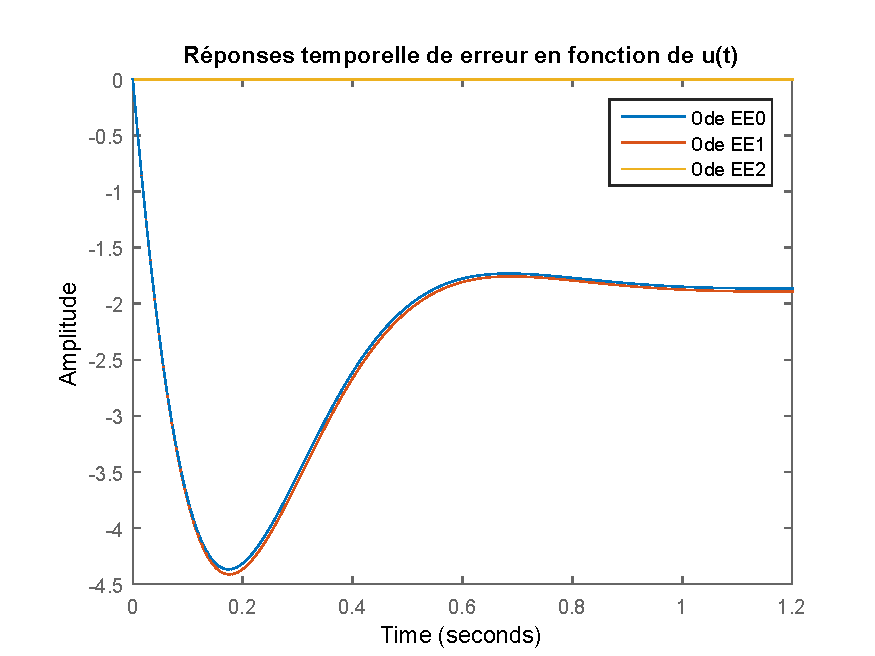
\includegraphics[width= .9\textwidth]{./III/figure/reponses_temp-erreurDeReconstruction.pdf}
\caption{\label{fig:repTemporelle_erreurReconstruction}Réponses de l'erreur de reconstruction de l'état $\omega$(vitesse) des modèle d'ordre 2 à 4}
\end{figure}Dans cette figure, nous voyons que l'erreur pour le modèle $EE2$ d'ordre 2, l'erreur converge très rapidement vers 0. Pour les autres modèles, l'erreur converge aussi, mais pas vers 0. Ce décalage du régime statique de $\epsilon$ ne nous permettra pas de reconstruire parfaitement l'état de la vitesse du moteur, mais uniquement de nous en approcher. 


\section{Simulation $SIMULINK$ des modèles linéaires}
Maintenant que l'observateur est prêt à être implémenter sur les modèles d'ordre 3 et 4, nous allons pouvoir commencer à exécuter des simulations des commandes de ces deux modèles. Deux choix s'offrent à nous, nous pouvons utilisé le changement de base et donc un système en espace d'état de notre système bouclé. Dans ce cas là, nous aurions accès à la vitesse asservis en fonction d'une référence. Le deuxième choix et celui qui nous semble le plus judicieux, consiste à brancher chaque élément sur un schéma $SIMULINK$. Nous avons ainsi accès à tous les échanges de signaux entre les blocs. Les schémas blocs que nous avons simulés sont disponibles en annexe \ref{Annex:SIMULINK_RE}. La réponse temporelle de $V_g(t)$ se trouve, pour les modèles linéaires d'ordre 2 à 3, dans la figure \ref{fig:reponseModelesLineairesSIMULINK}, ainsi que la commande qui est associé à cette réponse, en figure \ref{fig:reponseModelesLineairesSIMULINK}.
\begin{figure}[!ht]
\centering
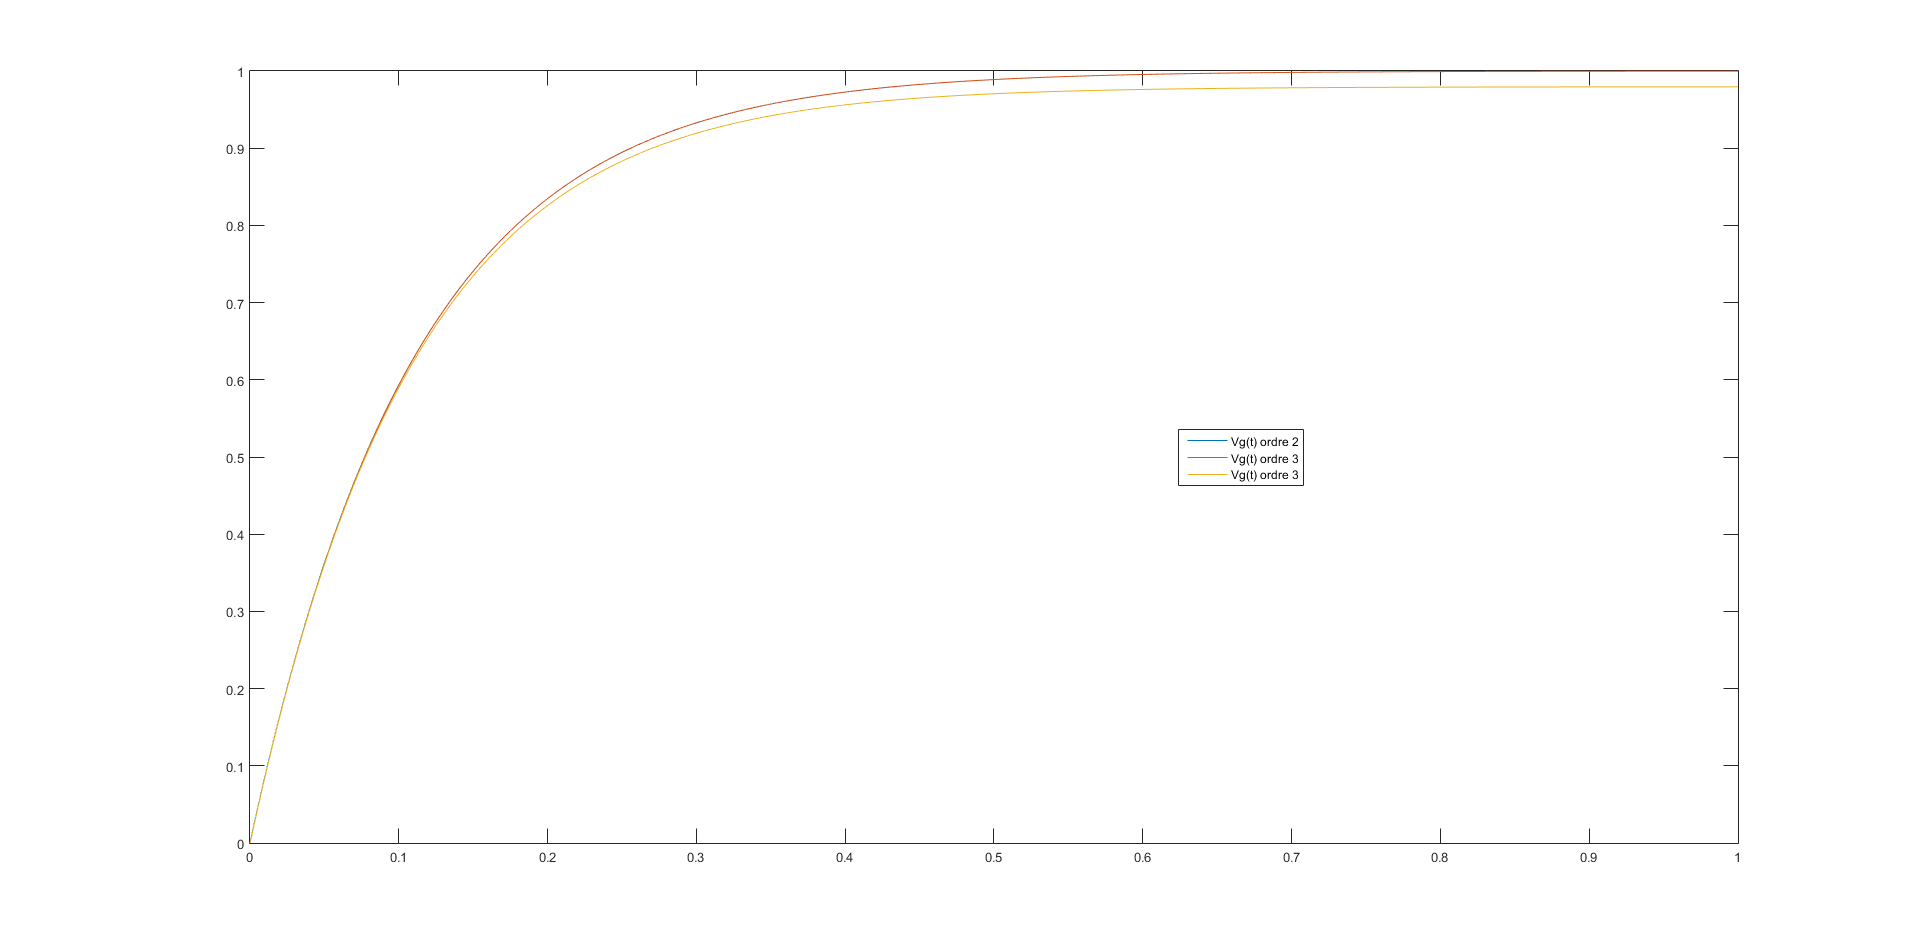
\includegraphics[scale=.3]{./III/figure/res_SIMULINK.png}
\caption{Réponses temporelles des boucles fermées sous $SIMULINK$\label{fig:reponseModelesLineairesSIMULINK}}
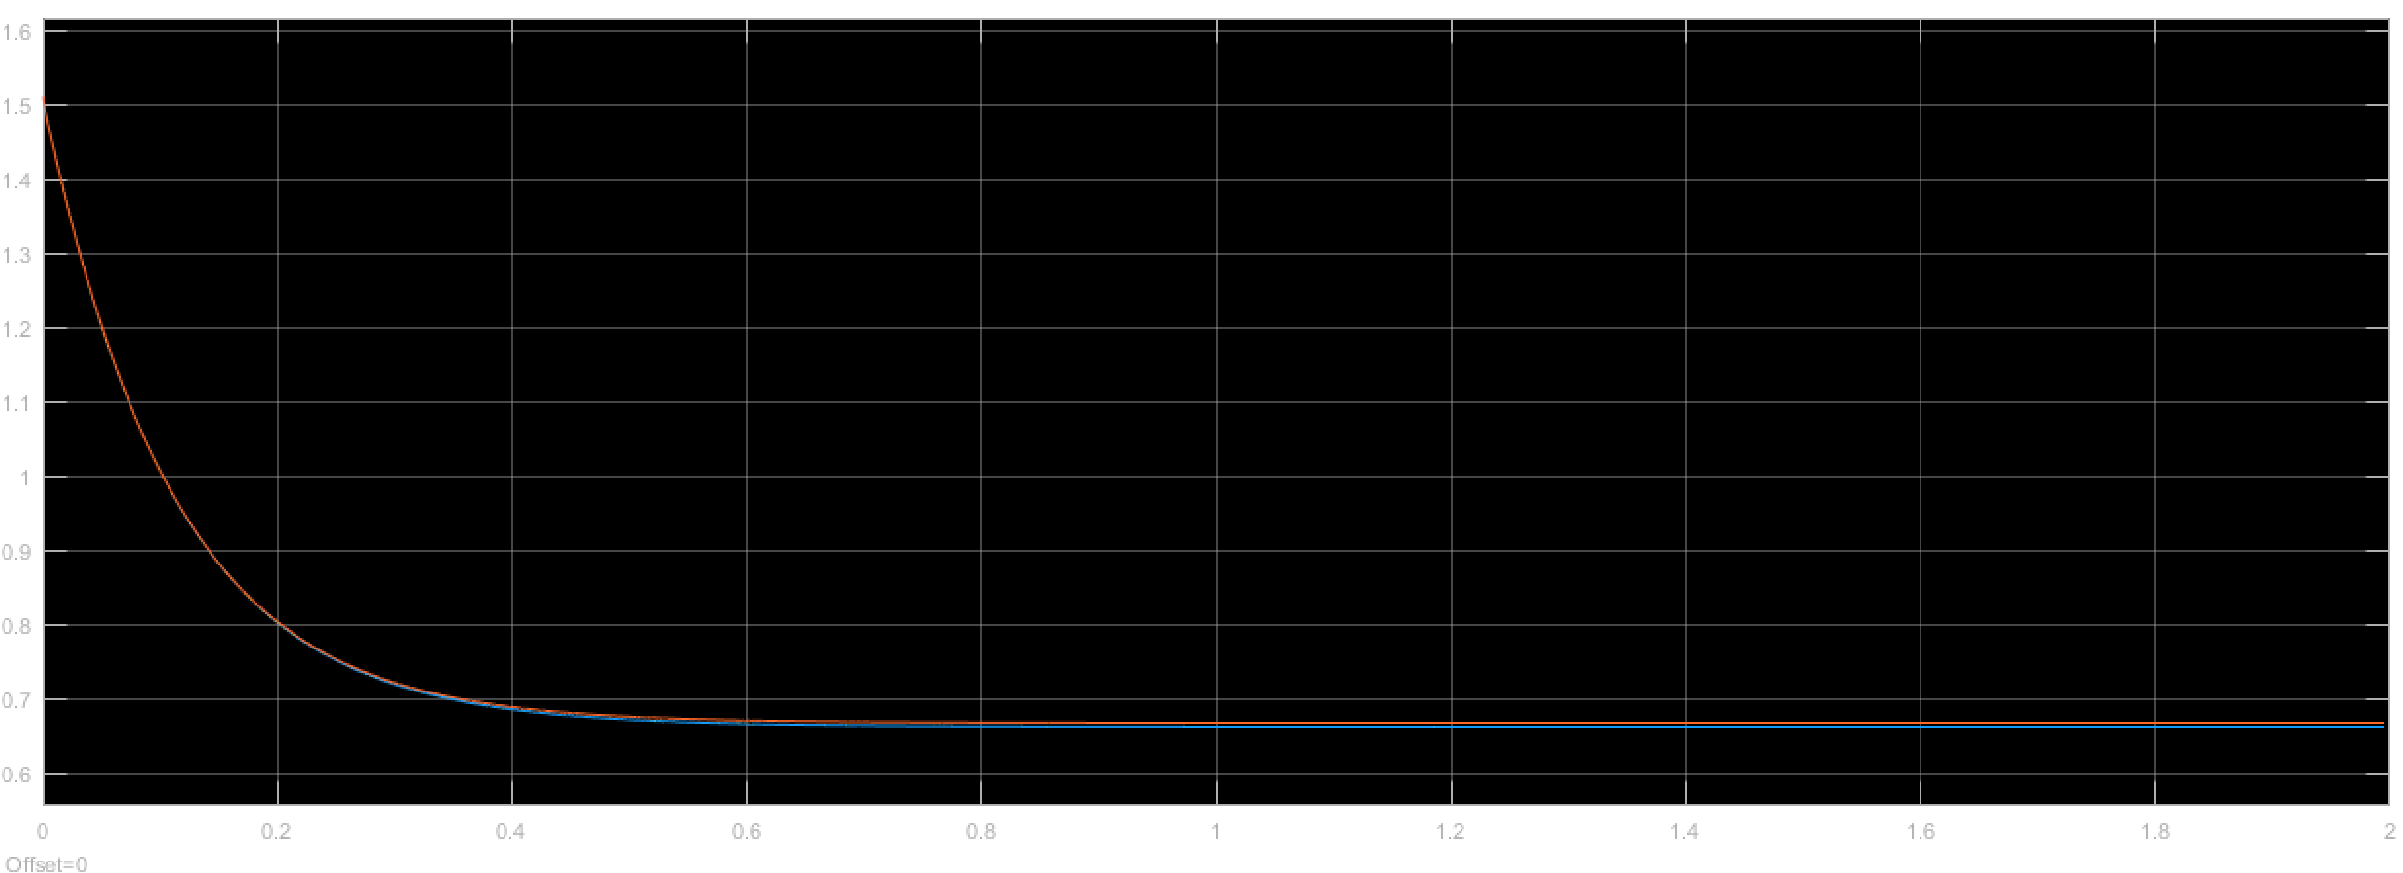
\includegraphics[scale=.4]{./III/figure/commande-u-ML_ordre2-3-4.pdf}
\caption{Commandes $u(t)$ associées aux résultats de la figure \ref{fig:reponseModelesLineairesSIMULINK}\label{fig:commandesML-1V}}
\end{figure}

Ces résultats nous permettent de regarder une simulation des signaux de $Vg(t)$. D'après ces résultats, la commande que nous souhaitons appliquer respecte le cahier des charges en termes d'oscillations de la réponse et de temps de réponse mais pas pour le gain statique. Cependant, nous ne pouvons en tirer aucune conclusion , il reste encore d'autres modèles plus complexes sur lequel notre commande doit être tester.




\chapter{Validation de la commande en temps continue sur le modèle non linéaire}\label{ValidationCommande}
Maintenant que les étapes de démonstration et d'émulation de la commande sont terminés, nous allons étudier notre premier prototype, que nous nommerons prototype 0, et qui correspondra  notre solution 0. Nous allons d'abord effectuer ce que nous appelons un \emph{Model in the loop} où nous allons chercher à améliorer ce premier prototype en utilisant uniquement des simulations. Par la suite, nous améliorerons le prototype en utilisation une technique d'émulation dite \emph{Software in the loop}.
\section{Protocoles MIL/SIL}
	\subsection{(MIL)}
	Pour faire une validation MIL, nous allons utiliser le modèle non linéaire pour simuler la correction. Toute cette opération sera effectué sous MATLAB à l'aide d'un bloc SIMULINK qui simule le modèle non linéaire. Pour valider le prototype de commande du correcteur, celui-ci devra respecter la ou les condition que nous lui imposerons. S'il ce n'est pas le cas, une amélioration de ce prototype sera nécessaire et elle nous permettra de créer un prototype N (pour N itérations de cette boucle). 
	Nous devons d'abord fixer une marge d'erreur par rapport au cahier des charges défini en \ref{chap:commande} : 
	\begin{align}\label{eqn_margeErreur}
		M_\epsilon < 1\%
	\end{align}
	Tant que notre prototype ne sera pas en dessous de cette marge, nous devrons le modifier et refaire le test.
	\subsection{SIL}
\section{Commande à temps continue}
	\subsection{Simulation}
		Nous disposons de la démarche que nous allons utiliser pour valider notre simulation. Pour cette partie, nous utiliserons un bloc SIMULINK qui nous permettra de simuler un modèle du Banc moteur très riche. Ce modèle n'a pas reçu les simplifications que posent les hypothèses faites en \ref{sub:linearisation} et en \ref{sub:invariance}.
		% Image et mesure
		\subsubsection{Adaptation modèle}
		% Encapsulation de la commande ?
		\subsubsection{Simulation et étude de performances}
		\subsubsection{Conclusion et Validation}
	\subsection{Sur moteur Réel}
		Nous souhaitons maintenant améliorer notre prototype avec le banc moteur directement. En utilisant la fonction de prototypage rapide de MATLAB, nous sommes capables de générer une émulation du micro contrôleur. Celui ci va s'occuper de récupérer les sorties mesurées du banc moteur, calculer la commande correspondantes et la générer sur l'entrée de commande du moteur. 
		\subsubsection{Adaptation du modèle}
		\subsubsection{Test et étude de performances}
		\subsubsection{Conclusion et Validation}
		
%\chapter{Planification de la suite de l'asservissement}
%\label{chap:suite}
%Dans ce chapitre, nous allons décrire les étapes suivantes à cette étude théorique. Dans un premier temps sera présenté la validation de notre commande par tests puis il sera abordé les étapes nécessaires à l'implémentation sur micro-contrôleur et la validation finale.
%\section{Validation de commande}
%Dans un premier temps, nous testerons notre asservissement sur un modèle plus riche (non linéaire, variant, plus de dynamique, ...) en simulation afin de voir si notre commande respecte toujours le cahier des charges. Le modèle sera fournie en seconde séance de TP. Ensuite, nous testerons le moteur dans différentes configurations en fonction des résultats et de notre vitesse d'avancement : 
%\begin{itemize}
%\item Émulation sur le même ordinateur (test du temps concret).
%\item Test de la commande et du procédé sur un même ordinateur en sortant le signal de commande par les cartes d'entrées/sorties du prototypage rapide.
%\item Test de la commande simulée sur un ordinateur et le procédé simulé sur un second ordinateur afin de tester deux vitesses de fonctionnement de simulation (synchronisations) et les cartes entrées/sorties (communications).
%\item Test de la commande simulée et le procédé simulé sur un micro-contrôleur.
%\item Test de la commande simulée sur procédé réel : on éprouve ici la robustesse de la commande face aux imprécisions de modélisation.
%\end{itemize}
%Nous effectuerons aussi une estimation du modèle de comportement du moteur que nous asservirons afin d'avoir un modèle plus proche du comportement réel.
%\section{Implémentation sur micro-contrôleur}
%% CAN CNA
%% Fech et F micro c
%% MODELE Z 
%% PROG
%% ORDO
%% IMPLE
%
%Dans cette partie, nous appréhenderons les problématiques de conversions de signaux numériques/analogiques et analogiques/numériques et essaierons de les corriger afin d'avoir des conversions les plus linéaires possibles. Nous calculerons les fréquences maximales et minimales des entrées et sorties du procédé, cela nous permettra de choisir des fréquences de conversions adaptées et la fréquence de fonctionnement du micro-contrôleur. Nous transformerons aussi notre modèle de commande en un modèle à temps discret afin de pouvoir l'implémenter. Une fois le modèle temps discret obtenu, nous programmerons les différentes fonctions nécessaires à l'asservissement (lecture des entrées, calcul des sorties, écriture des sorties). Nous aborderons aussi les problématiques d'ordonnancement afin que notre programme puisse s'exécuter dans le temps impartie afin de respecter les contraintes temps réels. Enfin, nous implémenterons notre programme sur le micro-contrôleur C167.
%\section{Validation finale}
%Une fois la commande implémentée, nous effectuerons les tests suivants : 
%\begin{itemize}
%\item Test de la commande implémentée sur le procédé simulé sur ordinateur.
%\item Test de la commande implémentée sur le procédé simulé sur micro-contrôleur.
%\item Test de la commande implémentée sur la maquette du procédé réel.
%\end{itemize}
%
%Nous vérifierons le respect des spécifications du cahier des charges dans l'ensemble de ces tests afin de voir si notre asservissement est correct.

%\chapter{Commande temps discret}
Afin d'implémenter la commande, nous avons dans un premier temps évaluer les contraintes lié au support d'implémentation et dans un second temps nous allons adapter la commande de façon à ce qu'elle soit implémentable sur le micro-contrôleur. Ensuite, nous évaluerons cette transformation. Voici, ci-dessous figure \ref{fig:GeneralSCHEMA}, le schéma général des différents éléments.	
\begin{figure}[!ht]
\centering 
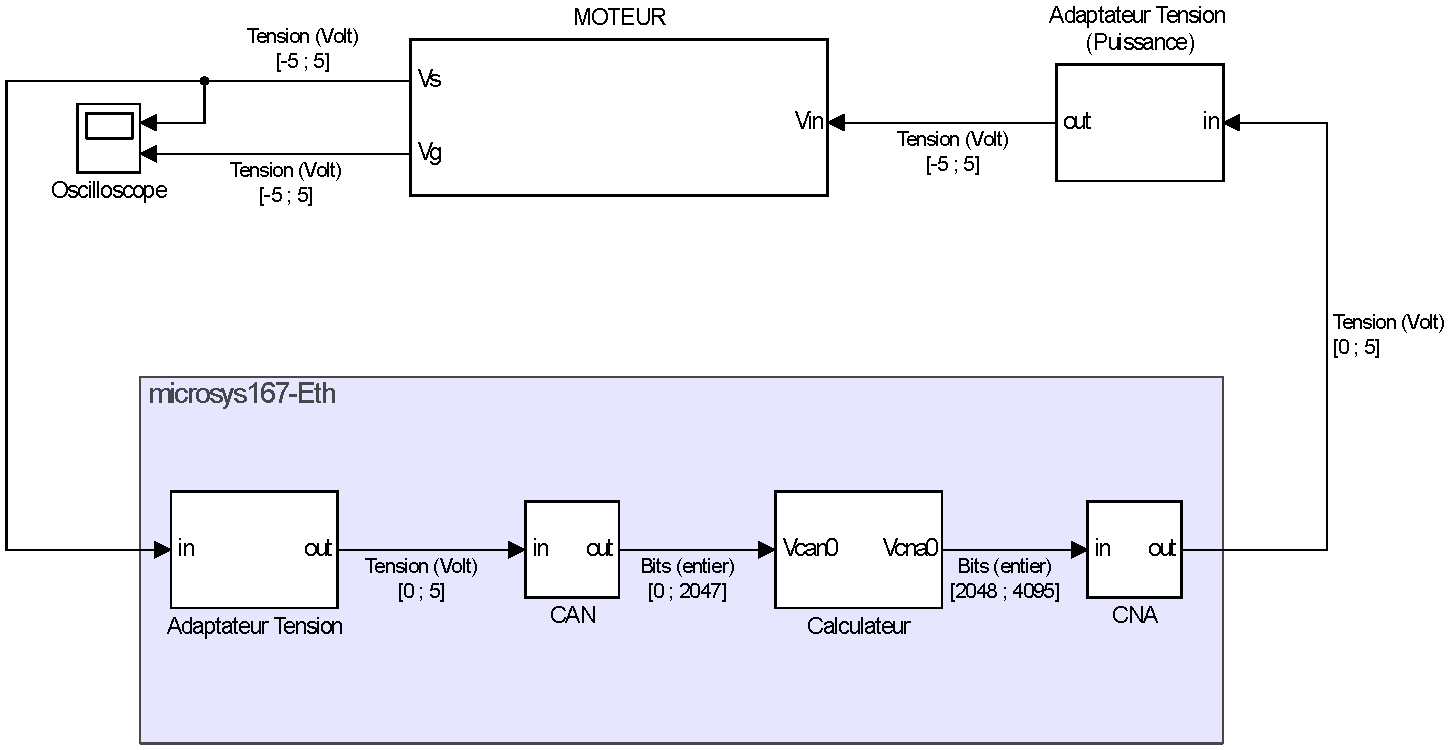
\includegraphics[width=.7\textwidth]{./V/images/schemaMO_MICRO.pdf}
\caption{\label{fig:GeneralSCHEMA}Schéma des différents composants du montage.}
\end{figure}
On remarque qu'il y a 4 composants et le détail, non exhaustif, des éléments utiles de la carte \emph{microsys167-Eth}.
Le bloc nommé moteur correspond au banc moteur présent en salle de TP. Le bloc adaptateur de tension (Puissance) est la carte qui permet de passer de la tension de commande ($0$ à $5$ Volt) vers une tension adaptée au moteur ($-5$ à $5$ Volt).
\section{Contraintes hardware} 
Nous allons, dans cette partie, nous consacrer à une étude des contraintes matérielles. Dans un premier temps nous verrons quels sont les spécificités du micro-contrôleur. Puis, nous verrons les convertisseurs analogique/numérique et numérique/analogique et nous conclurons sur le choix du micro-contrôleur. 
	\subsection{Micro-contrôleur C167}
		%(ordo,taches,validation TR,temps calcul, fréquence fonctionnement)
Pour ce projet, nous disposons d'un micro-contrôleur \emph{C167} fabriqué par Siemens. Il est dans une carte \emph{microsys167-Eth} qui lui  ajoute des interfaces, des fonctionnalités et de la mémoire. La carte cadence le micro-contrôleur à $20\text{ }MHz$, ajoute un $1\text{ }Mo$ de RAM et $512\text{ } Ko$ de Flash-EPROM. Nous disposons aussi d'adaptateurs de tension ($\left[-5;5\right]$ Volt vers $\left[0;5\right]$ Volt). Le \emph{C167} offre différentes fonctionnalités, dont les interruptions matérielles, les taches, les timers périodiques et un débogueur. Nous avons également des outils de développement permettant depuis un ordinateur, de créer un programme en \emph{C}, le compiler pour le \emph{C167}, l'envoyer sur celui-ci et si besoin de le déboguer et récupérer des valeurs sur un terminal. La fréquence de fonctionnement du \emph{C167} est de $20 $ MHz et un cycle instruction faut 4 cycle CPU, donc la fréquence d'instruction est de $5 $ MHz.
Le \emph{C167} a également des entrées et des sorties numériques et analogiques. Nous allons maintenant vous parlez des problématiques de conversions.
	\subsection{CAN / CNA}
%		(protocole correction, temps conversion, échantillonnage bits )	

%%%% CAN			
Nous allons détailler deux types de conversions nécessaires à ce projet. \\
\hspace{3mm} \textbf{CAN :} (Conversion Analogique Numérique.) Durant cette opération, le convertisseur échantillonne grâce à un bloqueur (discrétisation temporelle) puis quantifie (discrétisation de l'amplitude) le signal analogique. Il restitue un signal numérique après un temps de conversion $t_{CAN}$. Nous avons besoin de ce type de convertisseur pour la lecture des entrées dans notre cas, $V_{D}$. La qualité de notre conversion dépend de plusieurs éléments : 
\begin{itemize}
\item Le nombre de bits de sortie (la sortie ne pouvant prendre que $2^{\text{nbrBit}}$ valeurs différentes). Nous avons des CAN 11 bits.
\item La fréquence de conversion du signal analogique $f_{e}$ par rapport à la fréquence utile maximale du signal a convertir $f_{max}$. Le théorème de Shannon préconise d'avoir au moins le rapport de l'équation \ref{equ:Fshannon}, en pratique nous respecterons le rapport de l'équation \ref{equ:Freel}. Cela évite le repliement.
\begin{eqnarray}
\label{equ:Fshannon} f_e &>& 2*f_{max}\\
\label{equ:Freel} f_e & \approx & 10*f_{max}
\end{eqnarray}
Nous avons considéré que la fréquence utile maximale de la position d'un moteur à courant continue est d'environ $f_{max} = 100Hz$. Nous avons donc prendre $f_e = 1kHz$.
\item La conversion doit être linéaire. En effet, il existe différentes erreurs possibles. Il peut y avoir un offset, une erreur de gainn une non-linéarité intégrale ou différentielle (voir figure \ref{fig:errCAN}).
\end{itemize}
\begin{figure}[!ht]
\centering 
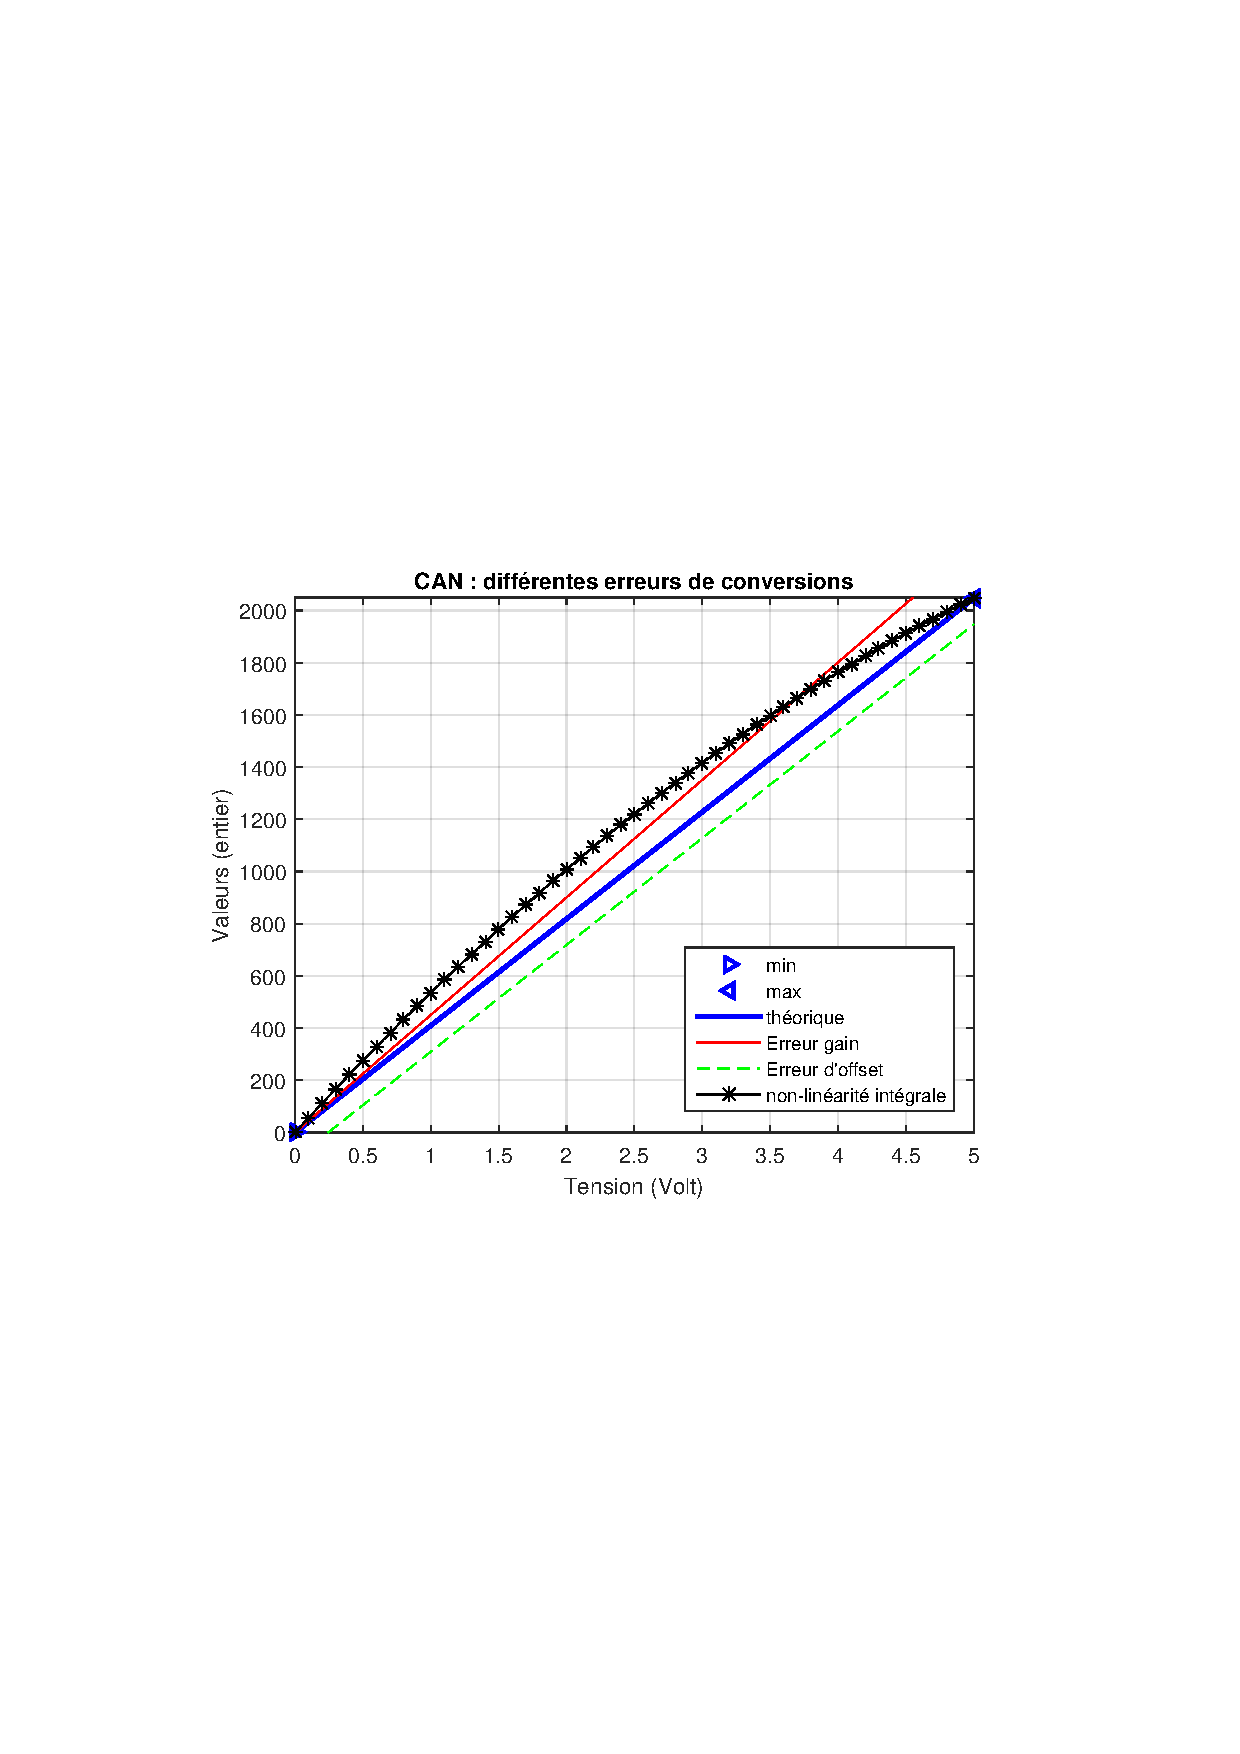
\includegraphics[width=.6\textwidth]{./V/images/CAN.pdf}
\caption{\label{fig:errCAN}Erreurs sur le CAN}
\end{figure}

%%%% CNA 
\hspace{3mm} \textbf{CNA :} (Conversion Numérique Analogique.) Ici, le convertisseur transforme le signal numérique en un signal analogique après un temps de conversion $t_{CNA}$. Nous avons besoin de ce type de convertisseur pour la génération de la sortie dans notre cas, $V_{s}$. La qualité de notre conversion dépend de plusieurs éléments similaires au CAN. L'entrée du CNA est un entier codé sur 12 bits et il génère une tension comprise entre $-5$ et $5$ Volts. 


Par manque de temps, nous n'avons pas eu le temps mettre en place un protocole complet d'étude des erreurs de conversions, nous avons uniquement vérifié que les valeurs mesurées et générées correspondent à celles désirées. Nous avons fait ceci pour quelques valeurs (min, max et milieu).

Un protocole de test complet aurait été :\\
\begin{itemize}
\item Pour le CAN : 
	\begin{itemize}
		\item Générer, à partir d'un générateur de basse tension, un signal triangle de $0$ à $5$ Volt de fréquence faible.
		\item Lire toutes les valeurs et les faire afficher sur un terminal par le micro-contrôleur.
		\item Les comparer (à l'aide d'un tableur ou de Matlab) et vérifier la linéarité de la conversion.
		\item À partir des ces résultats, créer une fonction qui corrige les erreurs, si possible.
	\end{itemize}

\item Pour le CNA :
	\begin{itemize}
		\item Générer, à partir du micro-contrôleur un signal triangle de $-5$ à $5$ Volt de fréquence faible.
		\item Récupérer les valeurs à partir d'un CAN déjà corrigé (carte d'acquisition Matlab, ou le CAN précédemment si la correction donne de très bons résultats).
		\item Les comparer (à l'aide d'un tableur ou de Matlab) et vérifier la linéarité de la conversion.
		\item À partir des ces résultats, créer une fonction qui corrige les erreurs, si possible.
	\end{itemize}
\end{itemize}
\begin{eqnarray}
T_{CAN} &=& 14*t_{cc} + 2*t_{sc} + 4*TLC \\
&=&  9,7 \mu s%\\
%T_{CNA} &=& %% TODO %%%%%%%%%%%%%%%%%%%%%%%%%%%%%%%%%%%%%%%%%%%%% /!\  %%%%%%%%%%%%%%%%%%%%%%%%%%%%%%%%%%%
\end{eqnarray}
%%%%%%%%%%%%%%%%%%%%%%%%%%%%%%%%%%%%%%%%%%%%% /!\  %%%%%%%%%%%%%%%%%%%%%%%%%%%%%%%%%%%
%%%%%%%%%%%%%%%%%%%%%%%%%%%%%%%%%%%%%%%%%%%%% /!\  %%%%%%%%%%%%%%%%%%%%%%%%%%%%%%%%%%%
%%%%%%%%%%%%%%%%%%%%%%%%%%%%%%%%%%%%%%%%%%%%% /!\  %%%%%%%%%%%%%%%%%%%%%%%%%%%%%%%%%%%\\
%%%%%%%%%%%%%%%%%%%%%%%%%%%%%%%%%%%%%%%%%%%%% /!\  %%%%%%%%%%%%%%%%%%%%%%%%%%%%%%%%%%%
	\subsection{Conclusion}
	  	(contraintes tempo, squelette code correcteur)
	  	
	  	
	  	

\section{Discrétisation de la commande}
	\subsection{Fonctions de transferts}
		 (observateur + retour état = 2 ft)
	\subsection{Transformée en z}

%\chapter{Implémentation}
\label{chap:implem}
Dans ce chapitre nous aborderons les problématiques lié à l'implémentation. Nous allons, dans un premier temps, évaluer les contraintes liés au support d'implémentation et dans un second temps les conversions que nous avons effectuer pour que l'entrée et la sortie de notre commande correspondent puissent être utilisé sur le micro-contrôleur. Finalement, nous expliquerons notre implémentation.\\

Voici, ci-dessous figure \ref{fig:GeneralSCHEMA}, le schéma général des différents éléments.	
\begin{figure}[!ht]
\centering 
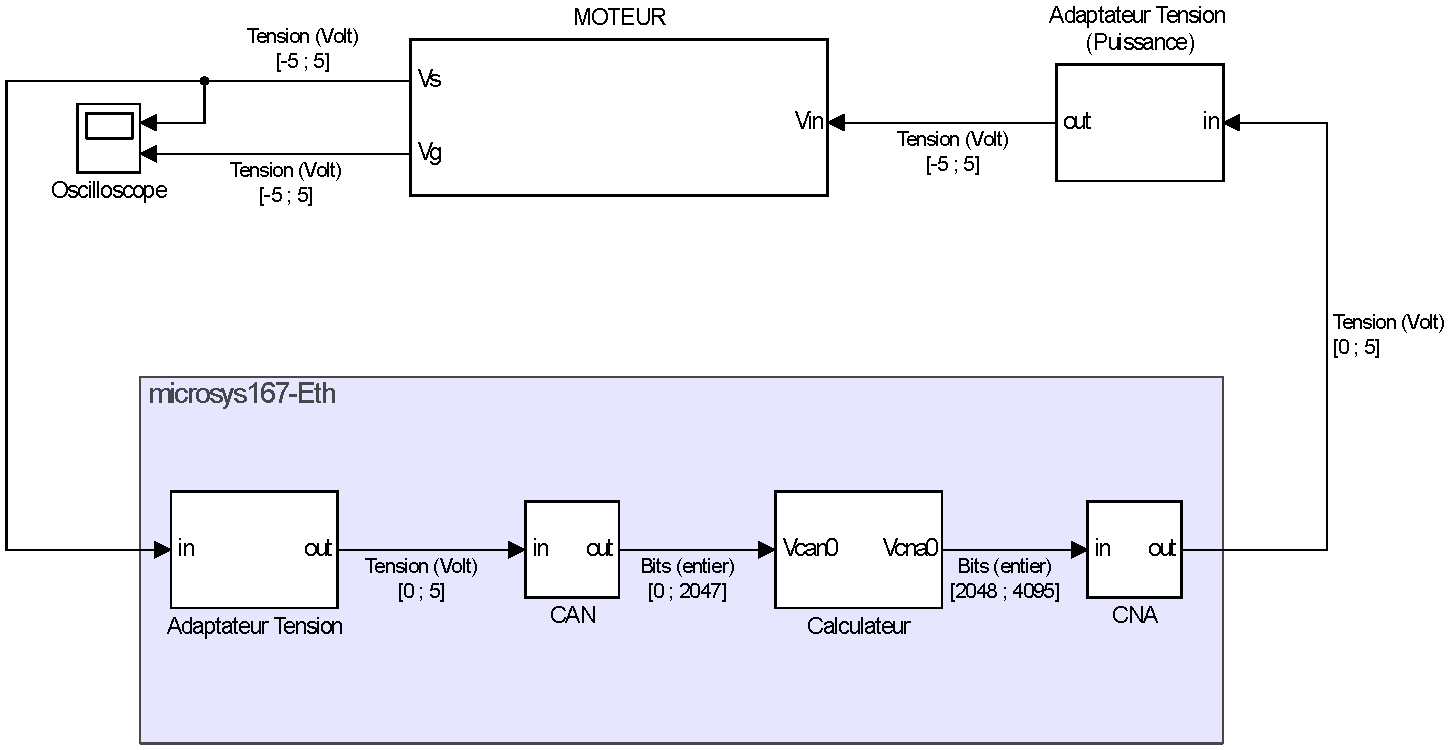
\includegraphics[width=.7\textwidth]{./V/images/schemaMO_MICRO.pdf}
\caption{\label{fig:GeneralSCHEMA}Schéma des différents composants du montage.}
\end{figure}
On remarque qu'il y a 4 composants et le détail, non exhaustif, des éléments utiles de la carte \emph{microsys167-Eth}.
Le bloc nommé moteur correspond au banc moteur présent en salle de TP. Le scope correspond à l'oscilloscope. Le bloc adaptateur de tension (Puissance) est la carte qui permet de passer de la tension de commande ($0$ à $5$ Volt) vers une tension adaptée au moteur ($-5$ à $5$ Volt).
\section{Contraintes hardware} 
Nous allons, dans cette partie, nous consacrer à une étude des contraintes matérielles. Dans un premier temps nous verrons quels sont les spécificités du micro-contrôleur. Puis, nous verrons les convertisseurs analogique/numérique et numérique/analogique et nous conclurons sur le choix du micro-contrôleur. 
	\subsection{Micro-contrôleur C167}
		%(ordo,taches,validation TR,temps calcul, fréquence fonctionnement)
Pour ce projet, nous disposons d'un micro-contrôleur \emph{C167} fabriqué par Siemens. Il est dans une carte \emph{microsys167-Eth} qui lui  ajoute des interfaces, des fonctionnalités et de la mémoire. La carte cadence le micro-contrôleur à $20\text{ }MHz$, ajoute un $1\text{ }Mo$ de RAM et $512\text{ } Ko$ de Flash-EPROM. Nous disposons aussi d'adaptateurs de tension ($\left[-5;5\right]$ Volt vers $\left[0;5\right]$ Volt). Le \emph{C167} offre différentes fonctionnalités, dont les interruptions matérielles, les taches, les timers périodiques et un débogueur. Nous avons également des outils de développement permettant depuis un ordinateur, de créer un programme en \emph{C}, le compiler pour le \emph{C167}, l'envoyer sur celui-ci et si besoin de le déboguer et récupérer des valeurs sur un terminal. La fréquence de fonctionnement du \emph{C167} est de $20 $ MHz et un cycle instruction faut 4 cycle CPU, donc la fréquence d'instruction est de $5 $ MHz.
Le \emph{C167} a également des entrées et des sorties numériques et analogiques. Nous allons maintenant vous parlez des problématiques de conversions.
	\subsection{CAN / CNA\label{sub:CAN_CNA}}
%		(protocole correction, temps conversion, échantillonnage bits )	
\subsubsection{CAN}
%%%% CAN			
Nous allons détailler deux types de conversions nécessaires à ce projet. \\
\hspace{3mm} \textbf{CAN :} (Conversion Analogique Numérique.) Durant cette opération, le convertisseur échantillonne grâce à un bloqueur (discrétisation temporelle) puis quantifie (discrétisation de l'amplitude) le signal analogique. Il restitue un signal numérique après un temps de conversion $t_{CAN}$. Nous avons besoin de ce type de convertisseur pour la lecture des entrées dans notre cas, $V_{D}$. La qualité de notre conversion dépend de plusieurs éléments : 
\begin{itemize}
\item Le nombre de bits de sortie (la sortie ne pouvant prendre que $2^{\text{nbrBit}}$ valeurs différentes). Nous avons des CAN 11 bits.
\item La fréquence de conversion du signal analogique $f_{e}$ par rapport à la fréquence utile maximale du signal a convertir $f_{max}$. Le théorème de Shannon préconise d'avoir au moins le rapport de l'équation \ref{equ:Fshannon}, en pratique nous respecterons le rapport de l'équation \ref{equ:Freel}. Cela évite le repliement.
\begin{eqnarray}
\label{equ:Fshannon} f_e &>& 2*f_{max}\\
\label{equ:Freel} f_e & \approx & 5*f_{max}
\end{eqnarray}
Nous avons considéré que la fréquence utile maximale de la position d'un moteur à courant continue est d'environ $f_{max} = 100Hz$. Nous avons donc pris :
\begin{eqnarray}
\label{equ:fe}f_e &=& 520\text{Hz}\\
\label{equ:Te} T_e &=& 52 \text{ms}\\
\end{eqnarray}
\item La conversion doit être linéaire. En effet, il existe différentes erreurs possibles. Il peut y avoir un offset, une erreur de gainn une non-linéarité intégrale ou différentielle (voir figure \ref{fig:errCAN}).
\end{itemize}
\begin{figure}[!ht]
\centering 
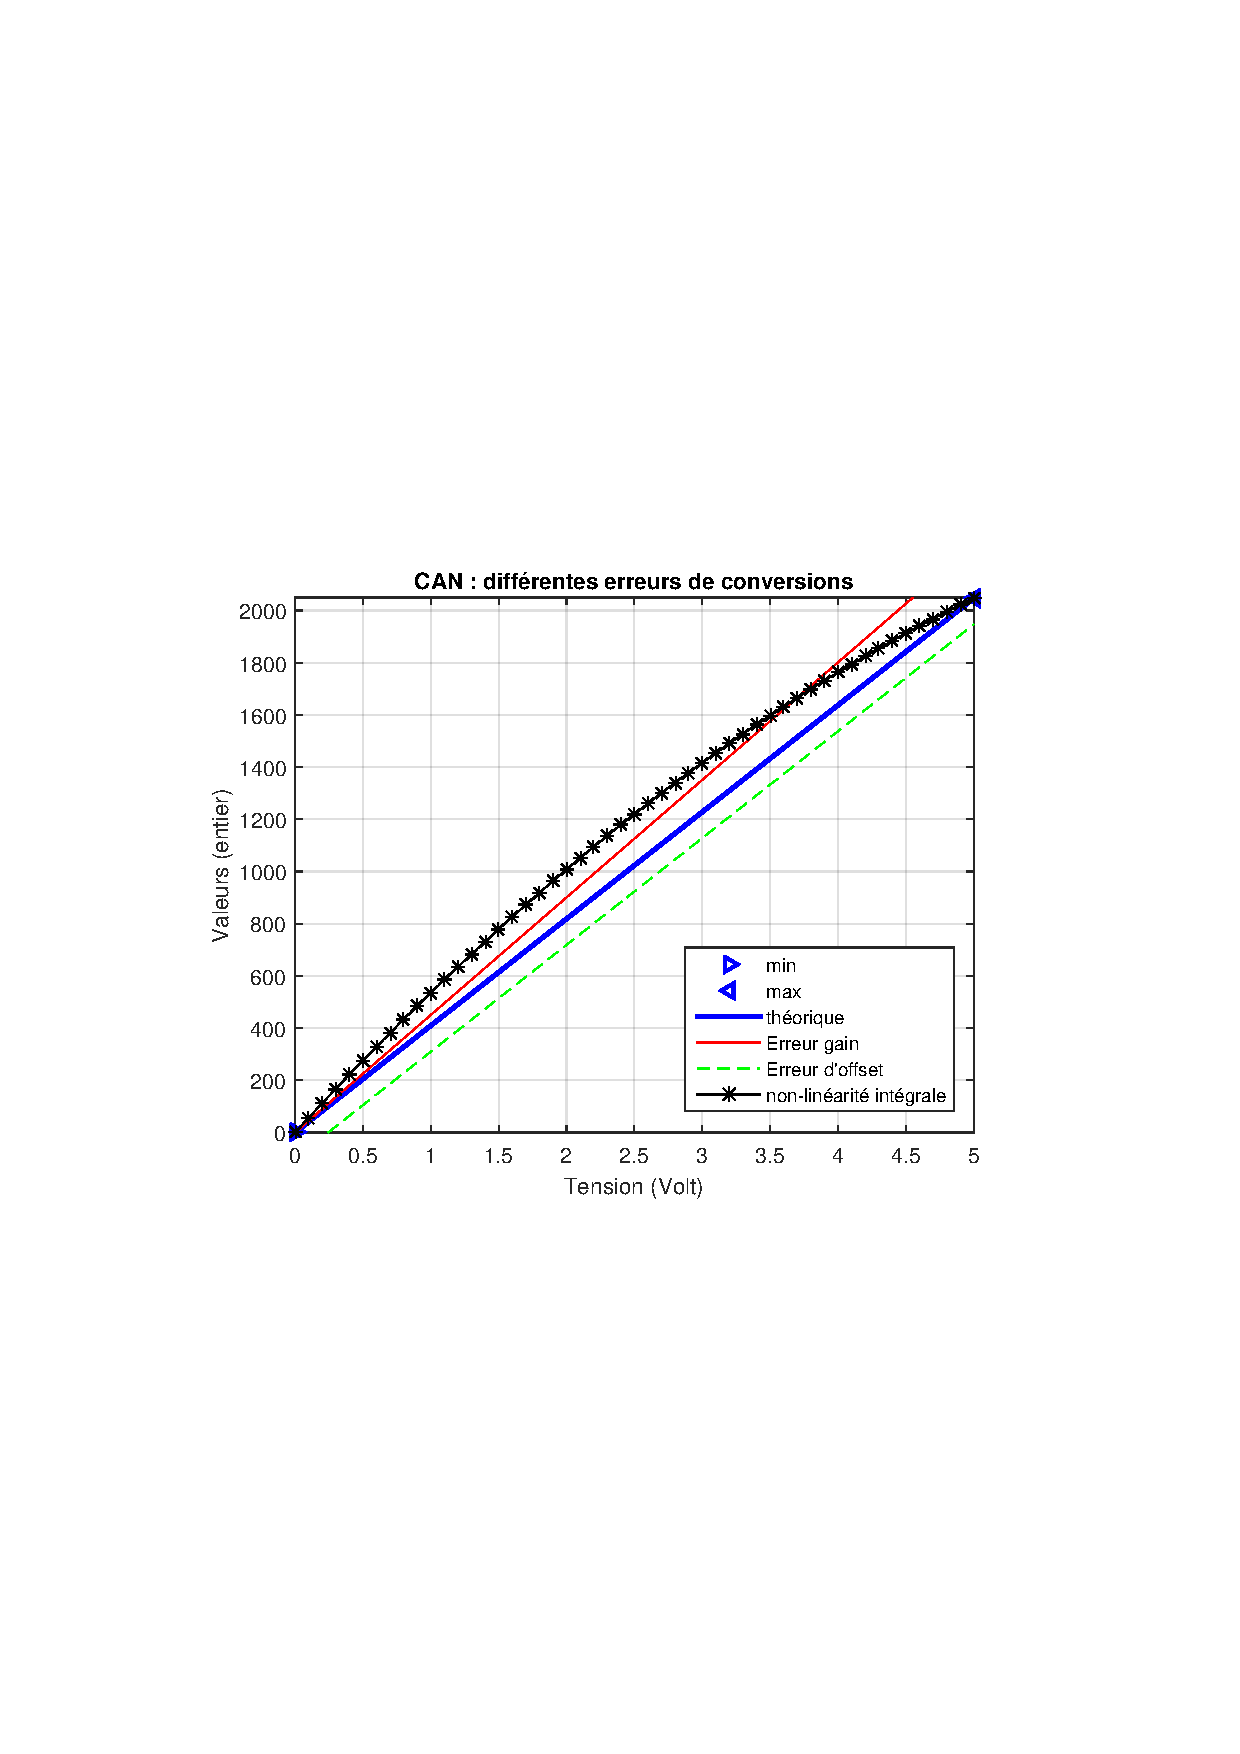
\includegraphics[width=.6\textwidth]{./V/images/CAN.pdf}
\caption{\label{fig:errCAN}Erreurs de conversions possibles sur le CAN}
\end{figure}
\subsubsection{CNA}
\hspace{3mm} \textbf{CNA :} (Conversion Numérique Analogique.) Ici, le convertisseur transforme le signal numérique en un signal analogique après un temps de conversion $t_{CNA}$ (équation \ref{equ:tcan}). Nous avons besoin de ce type de convertisseur pour la génération de la sortie dans notre cas, $V_{s}$. La qualité de notre conversion dépend de plusieurs éléments similaires au CAN. L'entrée du CNA est un entier codé sur 12 bits et il génère une tension comprise entre $-5$ et $5$ Volts. 
\begin{eqnarray}
\label{equ:tcan}
t_{CAN} &=& 14*t_{cc} + 2*t_{sc} + 4*TLC \\
&=&  9,7 \mu s%\\
%T_{CNA} &=& %% TODO %%%%%%%%%%%%%%%%%%%%%%%%%%%%%%%%%%%%%%%%%%%%% /!\  %%%%%%%%%%%%%%%%%%%%%%%%%%%%%%%%%%%
\end{eqnarray}

Par manque de temps, nous n'avons pas pu mettre en place un protocole complet d'étude des erreurs de conversions, nous avons uniquement émis des valeurs avec le CNA et les avons lu avec le CAN afin que les valeurs mesurées et générées correspondent à peu prés à celles désirées. Nous avons fait ceci pour 1000 valeurs. Nous avons réaliser ce test pour les deux micro-contrôleurs et cela donne des résultats différents. La figure \ref{fig:errCAN_1} est le résultat de l'analyse du micro-contrôleur de gauche en salle de TP. Nous voyons que la conversion est assez mauvaise, d'autres tests ont mis en évidence que le problème vient du CAN : de multiples lectures d'une tension constante donnent des résultats avec une variation importante, trop pour être du bruit numérique ou électromagnétique. Nous avons ré effectué le même test sur le second micro-contrôleur (celui de droite) et, figure \ref{fig:errCAN}, on remarque qu'il y a deux saturations : avant $E1$ et après $E2$. Entre les deux, la conversion est à peu près constante. Le second C167 est donc plus fiable en terme de lecture et d'écriture de tensions.


Cette approche présente l'avantage d'être rapide mais elle est néanmoins peu précise. En effet, les erreurs du CAN peuvent être masqués par celles du CNA et inversement. Elle ne permet pas de savoir d'où vient le problème, à moins d'effectuer d'autres expériences sur le CAN et/ou le CNA.
\begin{figure}[!ht]
\begin{minipage}[t]{.48\textwidth}

\centering 		
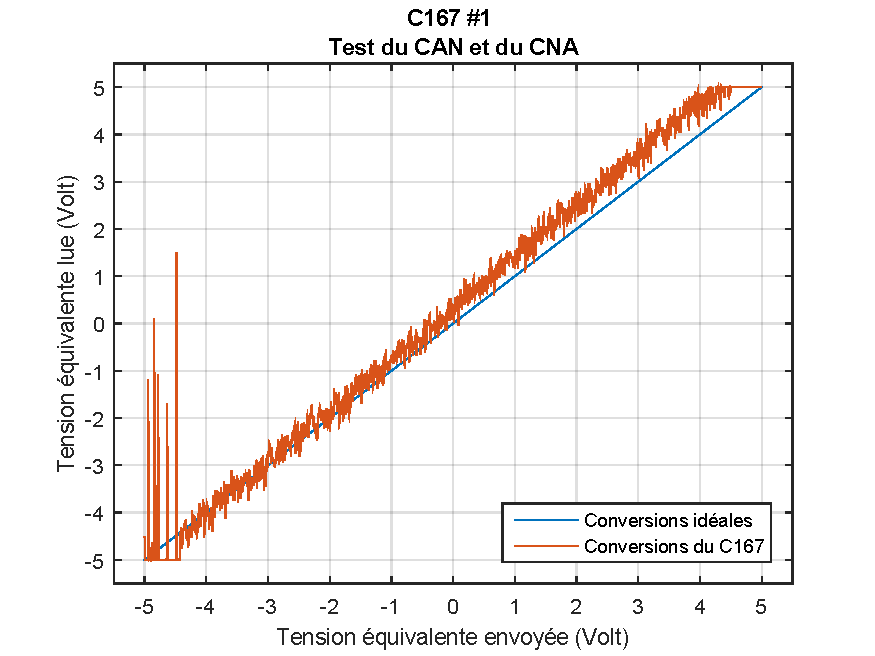
\includegraphics[width=.9\textwidth]{./V/images/CAN_CNA_mesures_1.pdf}
\caption{\label{fig:errCAN_1}Erreurs de conversions entre le CAN et le CNA (pour le C167 n°1)}
\end{minipage}\hfill%
\begin{minipage}[t]{.48\textwidth}
\centering 		
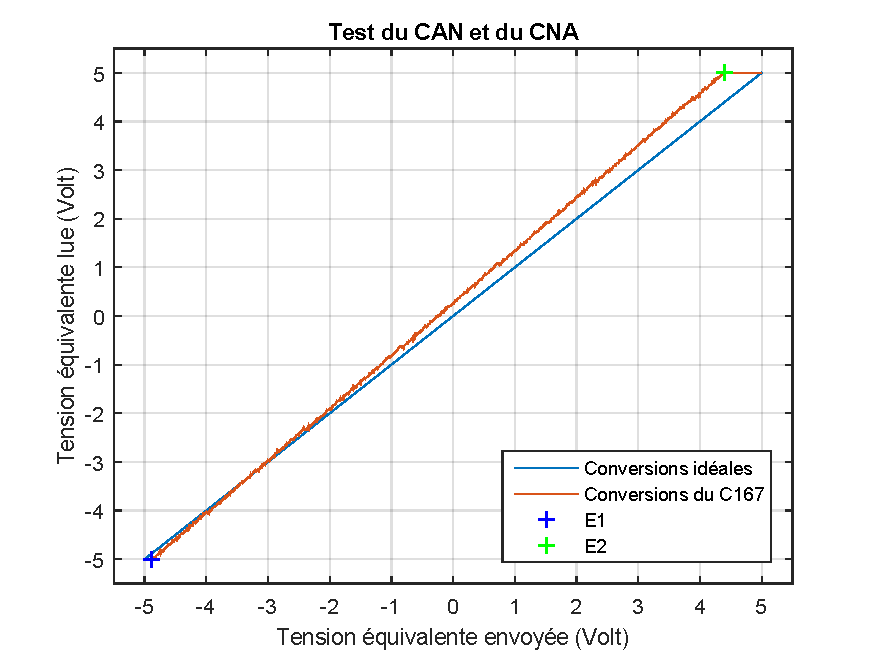
\includegraphics[width=.9\textwidth]{./V/images/CAN_CNA_mesures.pdf}
\caption{\label{fig:errCAN}Erreurs de conversions entre le CAN et le CNA (pour le C167 n°2)}
\end{minipage}
\end{figure}

Un protocole de test complet aurait été :\\
\begin{itemize}
\item Pour le CAN : 
	\begin{itemize}
		\item Générer, à partir d'un générateur de basse tension, un signal triangle de $0$ à $5$ Volt de fréquence faible.
		\item Lire toutes les valeurs et les faire afficher sur un terminal par le micro-contrôleur.
		\item Les comparer (à l'aide d'un tableur ou de Matlab) et vérifier la linéarité de la conversion.
		\item À partir des ces résultats, créer une fonction qui corrige les erreurs, si possible.
	\end{itemize}

\item Pour le CNA :
	\begin{itemize}
		\item Générer, à partir du micro-contrôleur un signal triangle de $-5$ à $5$ Volt de fréquence faible.
		\item Récupérer les valeurs à partir d'un CAN déjà corrigé (carte d'acquisition Matlab, ou le CAN précédemment si la correction donne de très bons résultats).
		\item Les comparer (à l'aide d'un tableur ou de Matlab) et vérifier la linéarité de la conversion.
		\item À partir des ces résultats, créer une fonction qui corrige les erreurs, si possible.
	\end{itemize}
\end{itemize}

%%%%%%%%%%%%%%%%%%%%%%%%%%%%%%%%%%%%%%%%%%%%% /!\  %%%%%%%%%%%%%%%%%%%%%%%%%%%%%%%%%%%
%%%%%%%%%%%%%%%%%%%%%%%%%%%%%%%%%%%%%%%%%%%%% /!\  %%%%%%%%%%%%%%%%%%%%%%%%%%%%%%%%%%%
%%%%%%%%%%%%%%%%%%%%%%%%%%%%%%%%%%%%%%%%%%%%% /!\  %%%%%%%%%%%%%%%%%%%%%%%%%%%%%%%%%%%\\
%%%%%%%%%%%%%%%%%%%%%%%%%%%%%%%%%%%%%%%%%%%%% /!\  %%%%%%%%%%%%%%%%%%%%%%%%%%%%%%%%%%%



\section{Transformation CAN/CNA}
\subsection{CAN}
Afin de réalisé notre commande, nous avons dût transformer la valeur entière lue pour $V_S$ par le CAN en un équivalent de la tension de type nombre à virgule flottante.  Figure \ref{fig:CAN_p}, nous pouvons observer les valeurs que peut convertir le CAN et les valeurs dont nous avons besoins. Nous n'utilisons ici que la moitié de la valeur lue par le convertisseur car nous n'avons besoin de convertir que des valeurs comprises entre $0$ et $5$ Volt. Ici, la plage de conversion est donc à moitié utilisée. 
Dans un premier temps, nous avons décaler la valeur lue (avec un et bit a bit) afin d'avoir la valeur sur $\left[ 0 , 1023\right]$,  puis  nous avons réalisé la conversion en tension avec l'équation \ref{equ:CAN1}.
\begin{figure}[!ht]%
\begin{minipage}{.5\textwidth}%
\centering
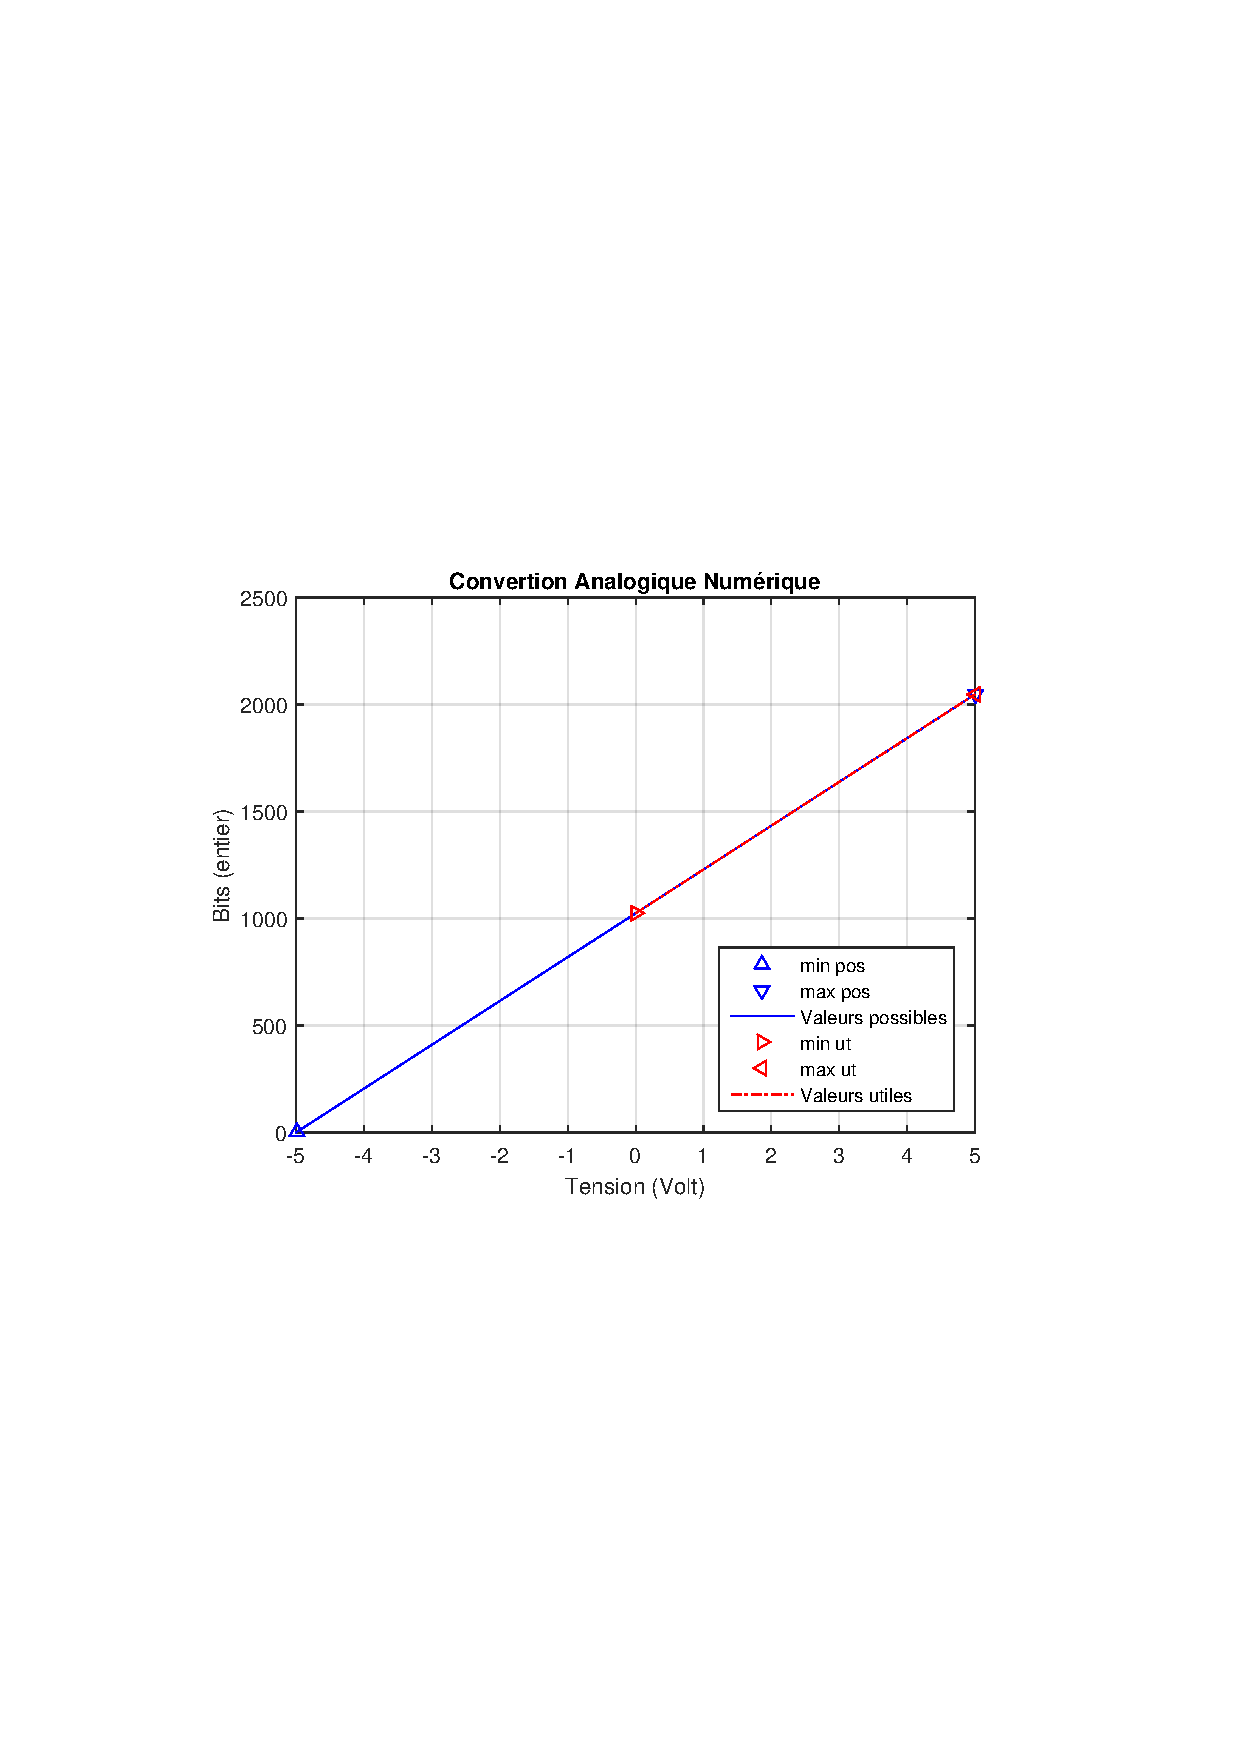
\includegraphics[width=\textwidth]{./VI/images/CAN_plage.pdf}
\caption{\label{fig:CAN_p}Valeurs possibles et possibles du CAN}
\end{minipage}%
\hfill%
\begin{minipage}{.5\textwidth}%
\begin{equation}
\begin{array}{l}
\left\lbrace
\begin{array}{lcl}
\label{equ:CAN1}V_{CANr} &=& V_{CAN} \&_{bàb} 1023\\
V_{volt} &=& \frac{5}{2^{10}-1}V_{CANr}
\end{array}
\right.\\
\Rightarrow V_{volt} = \frac{5}{2^{10}-1}( V_{CAN} \&_{bàb} 1023)
\end{array}
\end{equation}
\end{minipage}%
\end{figure}



\subsection{CNA}
La génération de la sortie $V_M$ nécessite aussi une conversion du CNA depuis la tension calculée par la commande (nombre à virgule flottante) vers un entier compris entre $-5$ et $5$ Volts. Néanmoins, la commande calcule une valeur comprise entre $-5$ et $5$ Volts, mais la carte de puissance branchée sur la sortie du CNA nécessite en entrée une tension comprise entre $0$ et $5$ Volt. Il faut donc, dans un premier temps, redresser la valeur calculée $V_{com}$ par la sortie sur une intervalle $\left[0;5\right]$ $V_{redr}$, puis le convertir en entier $V_{CNA}$. Pour cela nous utilisons les équations suivantes :

\begin{figure}[!ht]%
\begin{minipage}{.5\textwidth}%
\begin{equation}\label{eqn:CNA1}
\begin{array}{l}
\left\lbrace
\begin{array}{lcl}
V_{red}	&=&	\frac{1}{2}V_{com}+2,5\\
V_{CNA} &=& \frac{2^{11}-1}{5}V_{red}+2048\\
\end{array}
\right.\\
\Rightarrow V_{CNA} = \left\lfloor 204.7 V_{com} + 3071.5 \right\rfloor
\end{array}
\end{equation}	
\end{minipage}%
\hfill%
\begin{minipage}{.5\textwidth}%
\centering
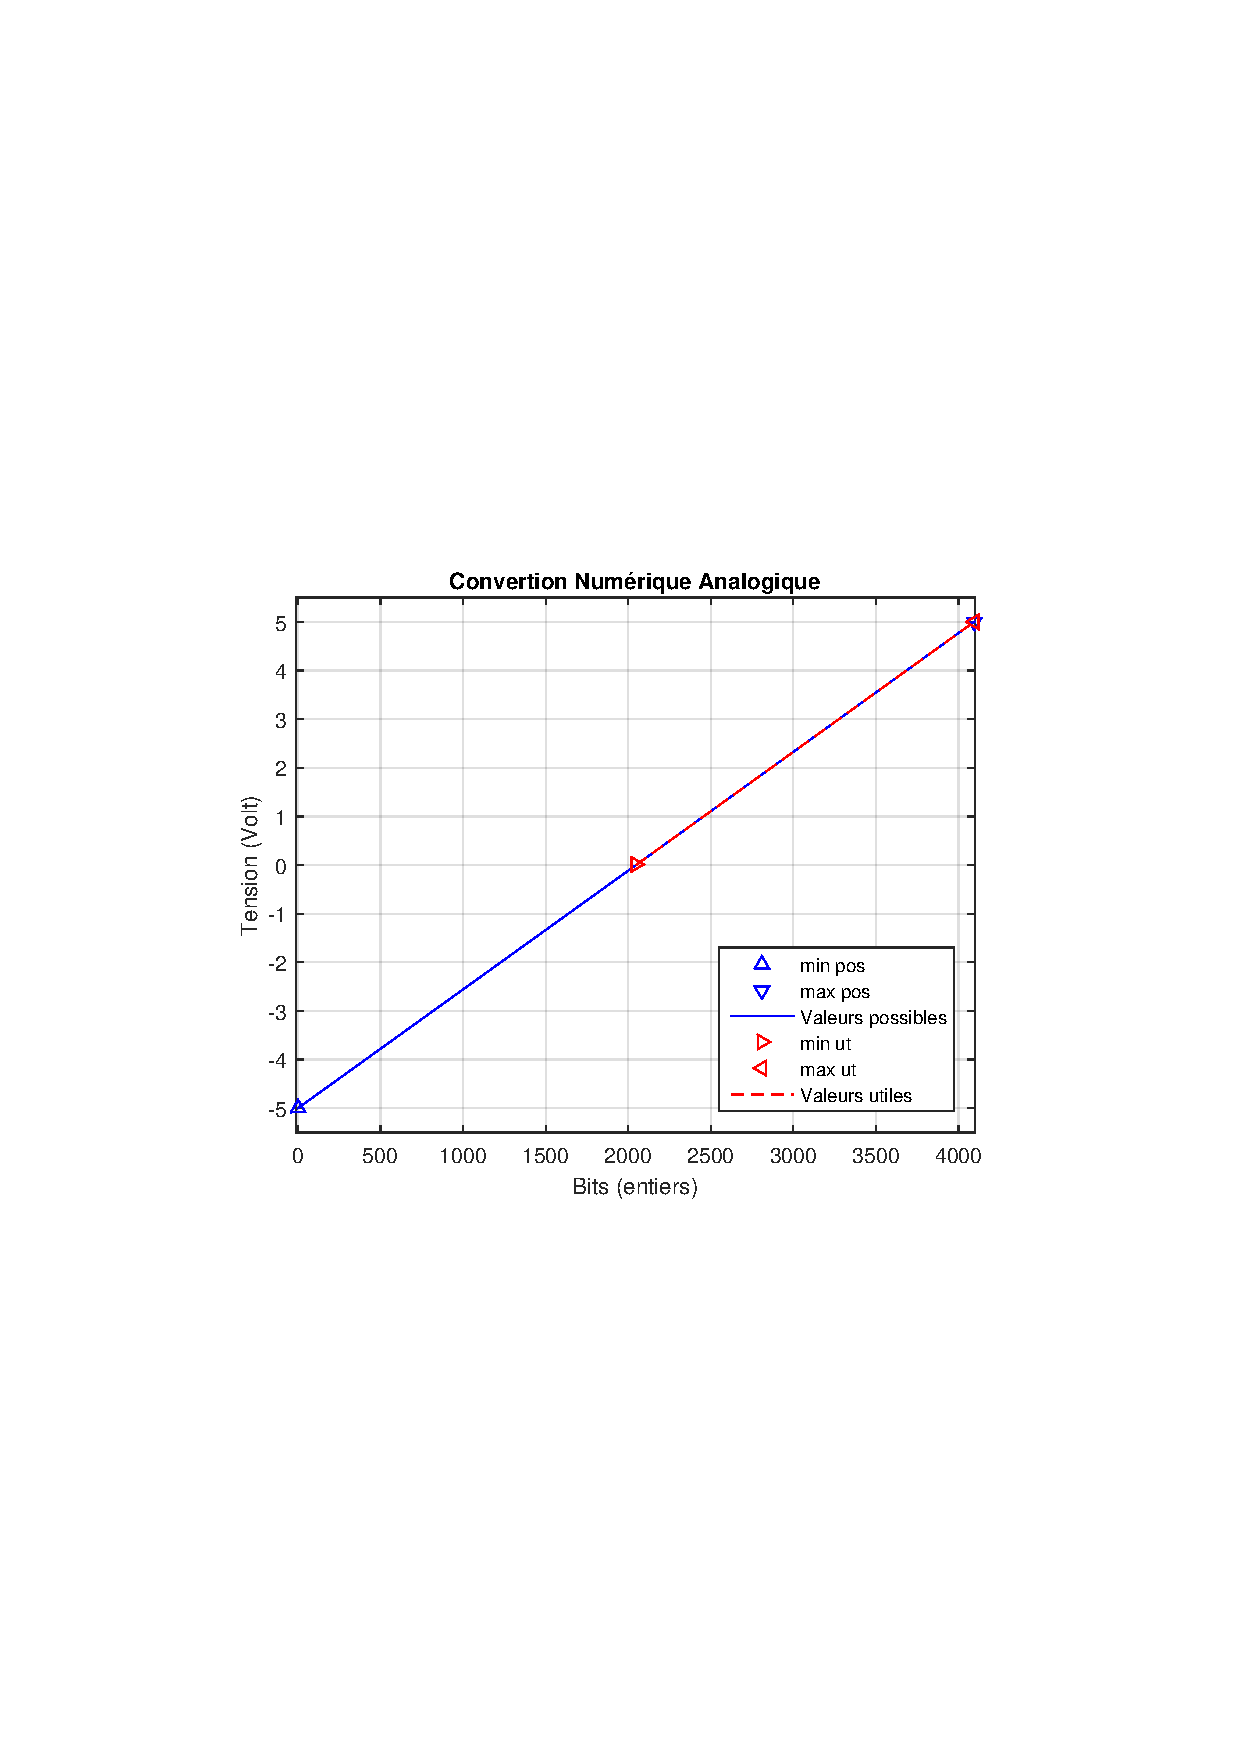
\includegraphics[width=\textwidth]{./VI/images/CNA_plage.pdf}
\caption{\label{fig:CNA_p}Valeurs possibles et possibles du CNA}
\end{minipage}%
\end{figure}

%	\subsection{Implémentation d'un programme de test des convertisseurs}
%	\subsection{Correction}
\section{Implémentation sur micro-contrôleur}	
Nous souhaitons dans cette partie vous présenter comment nous avons aborder l'implémentation des commandes sur le micro-contrôleur. Nous aborderons dans un premier temps une revue des tâches que nous avons utilisées. 
		\subsection{Description des taches}
		\paragraph*{Génération échelon}
		Une première tâche sera dédié à la génération d'un échelon. Nous souhaitons observer des changements de front de la consigne, c'est pourquoi il est intéressant de faire évoluer cette consigne périodiquement. Dans cette tâche, qui déroule du squelette obtenu sur les fichiers sources, nous allons avoir le déroulement suivant : \begin{itemize}
		\item[État 1] Valeur de la consigne mise à l'état haut. Variable d'état = 2
		\item[État 2] Valeur de la consigne mise à l'état bas. Variable d'état = 1
\end{itemize}
La fréquence d'appel de cette tâche n'a pas de grand impact sur les contraintes temps réel. Les timers ont déjà été programmé sur une fréquence de $f_{ech} = \frac{3.36}{2}Hz$, nous garderons ce résultat dans le reste de l'étude.		 
\paragraph{Acquisition des mesures}		 
		Cette tâche beaucoup plus principale que la précédente doit permettre de récupérer la valeur lue sur le CAN, calculer la commande associée et la transmettre au CNA. Ce déroulement a été décrit dans le schéma \ref{fig:GeneralSCHEMA}. Il est important de faire attention au conversion obtenu dans les équations \ref{eqn:CNA1} et \ref{equ:CAN1}.
		%	Acquisition 
		%	ref : CAN/CNA
		%         Conversion
		\subsection{Implémentation}
		Vous trouverez le code implémenté en langage C des tâches dans l'annexe \ref{Annex:codeC}. Nous avons aussi inclus un fichier de génération de paramètres via un modèle discret de $MATLAB$. Ce fichier génère un \emph{.txt} en fonction des paramètres de l'équation récurrente du prototype de commande.
		\subsection{Validation et correction}
		Nous avons obtenu des problèmes pour le prototype qui a été discrétisé dans la partie \ref{chap:Command} et qui est contenu dans le programme. Il semble que certaines problématiques nous ait échappé, notamment les notions de correction des CAN CNA évoquée dans \ref{sub:CAN_CNA}. Pour évaluer si le problème venait de la conversion, nous avons tout de même été capable de générer un échelon de tension qui vous est présenté dans la figure ci dessous. 
		\begin{figure}[!ht]
		\centering
		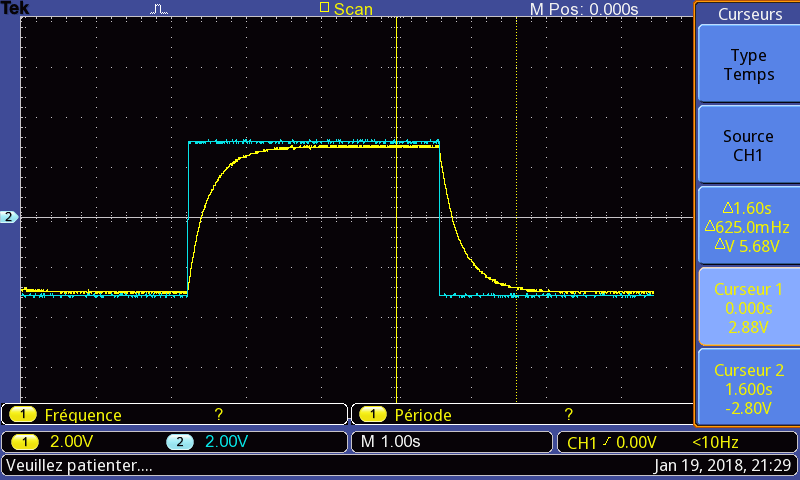
\includegraphics[width = .7\textwidth]{./VI/images/MicroC-reponseEchelon.png}
		\caption{Réponse à un échelon +2V, -2V}
\end{figure}				
		

%\input{./conclusions/conclusions.tex}

%\chapter{Bilan }

%Ne pas numéroter cette partie
\part*{Annexes}
%Rajouter la ligne "Annexes" dans le sommaire
\addcontentsline{toc}{part}{Annexes}

\chapter*{Annexe 1 - TITRE}
\addcontentsline{toc}{chapter}{TITRE}
%\setcounter{section}{0}
% **********************************
\addcontentsline{toc}{section}{TITRE}
\label{Annex:NOM_FICHIER}
\lstset{
  language=Matlab,                	  % choose the language of the code
  basicstyle=\ttfamily,
  numbers=left,                   % where to put the line-numbers
  stepnumber=1,                   % the step between two line-numbers.
  numbersep=5pt,                  % how far the line-numbers are from the code
  backgroundcolor=\color{white},  % choose the background color. You must add \usepackage{color}
  commentstyle = \color{darkgreen},
  showspaces=false,               % show spaces adding particular underscores
  showstringspaces=false,         % underline spaces within strings
  showtabs=false,                 % show tabs within strings adding particular underscores
  tabsize=2,                      % sets default tabsize to 2 spaces
  captionpos=b,                   % sets the caption-position to bottom
  breaklines=true,                % sets automatic line breaking
  breakatwhitespace=true,         % sets if automatic breaks should only happen at whitespace
  %caption=exo1.m,                 % show the filename of files included with \lstinputlisting;
  literate={á}{{\'a}}1 {è}{{\`e}}1 {é}{{\'e}}1,
}
%\lstinputlisting{./annexes/annexe1/NOMFICHIER.m} %{language = MAtlab}
\chapter*{Annexe 2 - Modèles SIMULINK}
\addcontentsline{toc}{chapter}{Modèles SIMULINK}
%\setcounter{section}{0}
% **********************************
\label{Annex:SIMULINK_RE}
\lstset{
  language=Matlab,                	  % choose the language of the code
  basicstyle=\ttfamily,
  numbers=left,                   % where to put the line-numbers
  stepnumber=1,                   % the step between two line-numbers.
  numbersep=5pt,                  % how far the line-numbers are from the code
  backgroundcolor=\color{white},  % choose the background color. You must add \usepackage{color}
  commentstyle = \color{darkgreen},
  showspaces=false,               % show spaces adding particular underscores
  showstringspaces=false,         % underline spaces within strings
  showtabs=false,                 % show tabs within strings adding particular underscores
  tabsize=2,                      % sets default tabsize to 2 spaces
  captionpos=b,                   % sets the caption-position to bottom
  breaklines=true,                % sets automatic line breaking
  breakatwhitespace=true,         % sets if automatic breaks should only happen at whitespace
  %caption=exo1.m,                 % show the filename of files included with \lstinputlisting;
  literate={á}{{\'a}}1 {è}{{\`e}}1 {é}{{\'e}}1,
}

\addcontentsline{toc}{section}{Modèle Global}
\section*{Modèle Global}
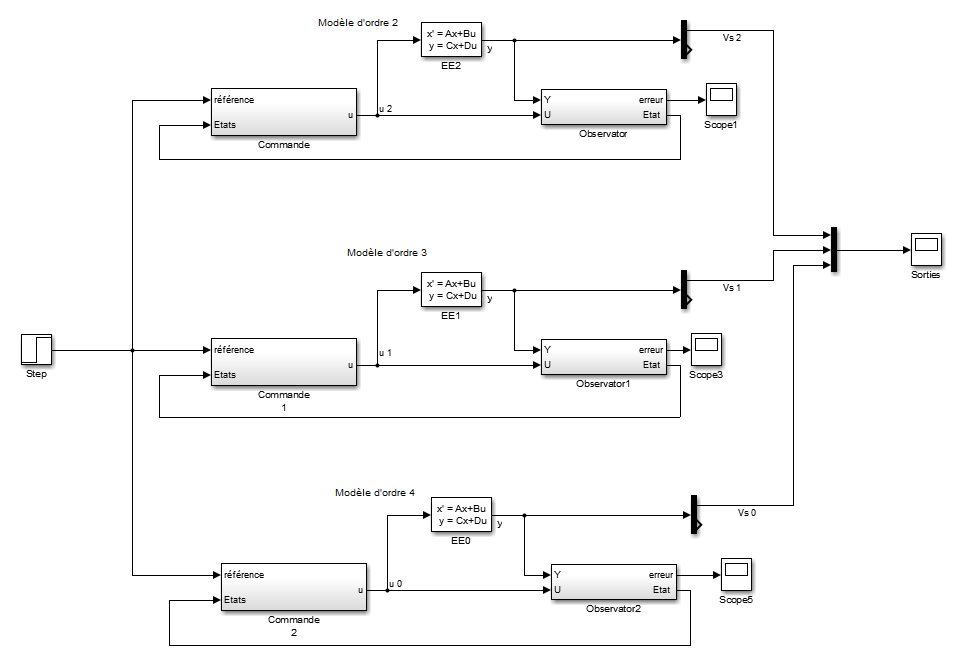
\includegraphics[width = \textwidth]{./annexes/annexe2/simu.PNG}

\addcontentsline{toc}{section}{Sous-système de commande}
\section*{Sous-système de commande}
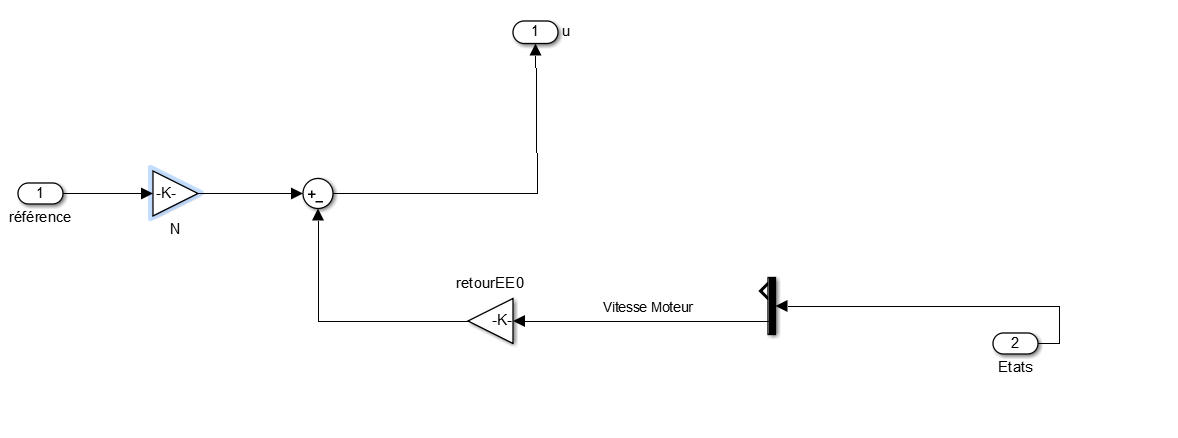
\includegraphics[width = \textwidth]{./annexes/annexe2/Command.PNG}

\addcontentsline{toc}{section}{Sous-système d'observateur}
\section*{Sous-système d'observateur}
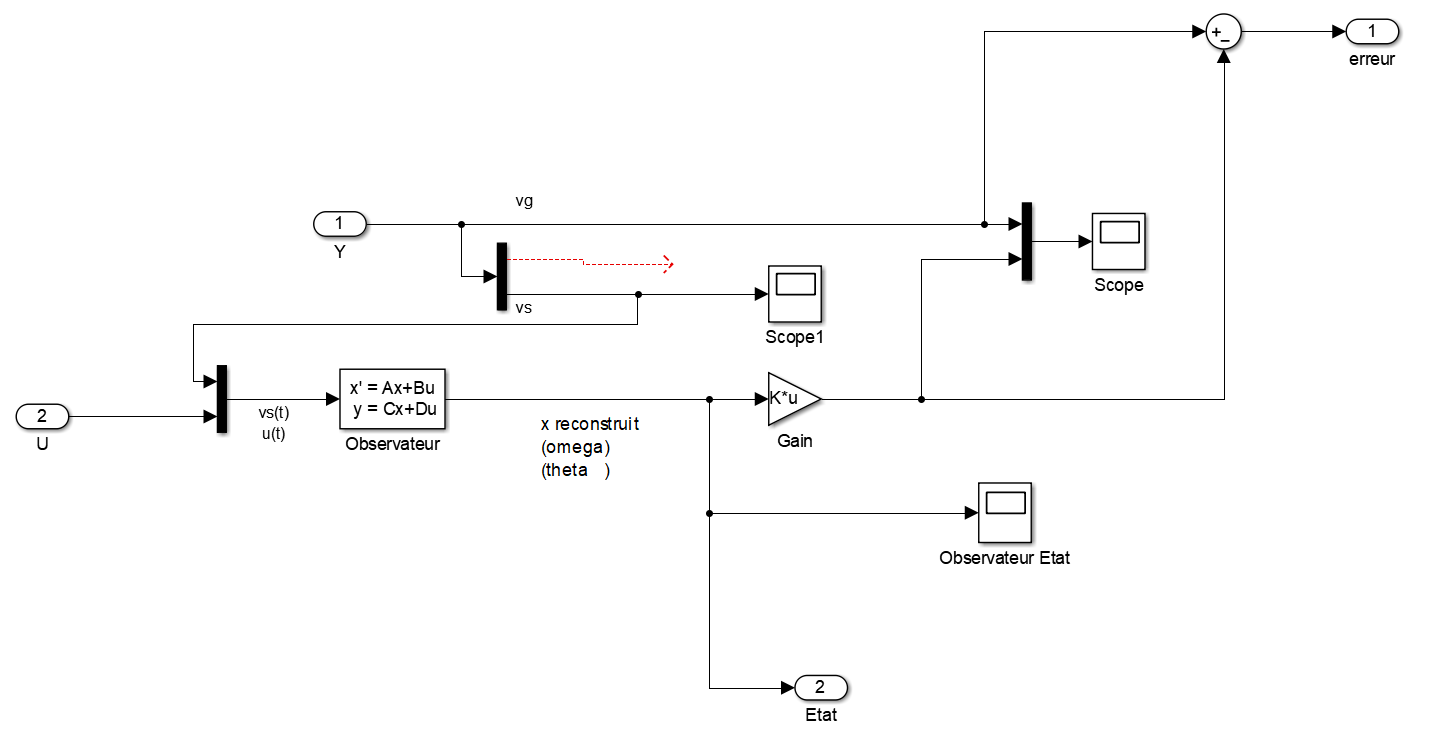
\includegraphics[width = \textwidth]{./annexes/annexe2/Observateur.PNG}	
\chapter*{Annexe 3 - Simulation \emph{SIMULINK}}
\addcontentsline{toc}{chapter}{Simulation \emph{SIMULINK}}
%\setcounter{section}{0}
% **********************************

%\label{Annex:SIMULINK_RE}
\lstset{
  language=Matlab,                	  % choose the language of the code
  basicstyle=\ttfamily,
  numbers=left,                   % where to put the line-numbers
  stepnumber=1,                   % the step between two line-numbers.
  numbersep=5pt,                  % how far the line-numbers are from the code
  backgroundcolor=\color{white},  % choose the background color. You must add \usepackage{color}
  commentstyle = \color{darkgreen},
  showspaces=false,               % show spaces adding particular underscores
  showstringspaces=false,         % underline spaces within strings
  showtabs=false,                 % show tabs within strings adding particular underscores
  tabsize=2,                      % sets default tabsize to 2 spaces
  captionpos=b,                   % sets the caption-position to bottom
  breaklines=true,                % sets automatic line breaking
  breakatwhitespace=true,         % sets if automatic breaks should only happen at whitespace
  %caption=exo1.m,                 % show the filename of files included with \lstinputlisting;
  literate={á}{{\'a}}1 {è}{{\`e}}1 {é}{{\'e}}1,
}
\section*{Modèles Non linéaire}\label{annex:modl_NL_SIMULINK}
\addcontentsline{toc}{section}{Modèles Non linéaire}
\begin{figure}
\centering
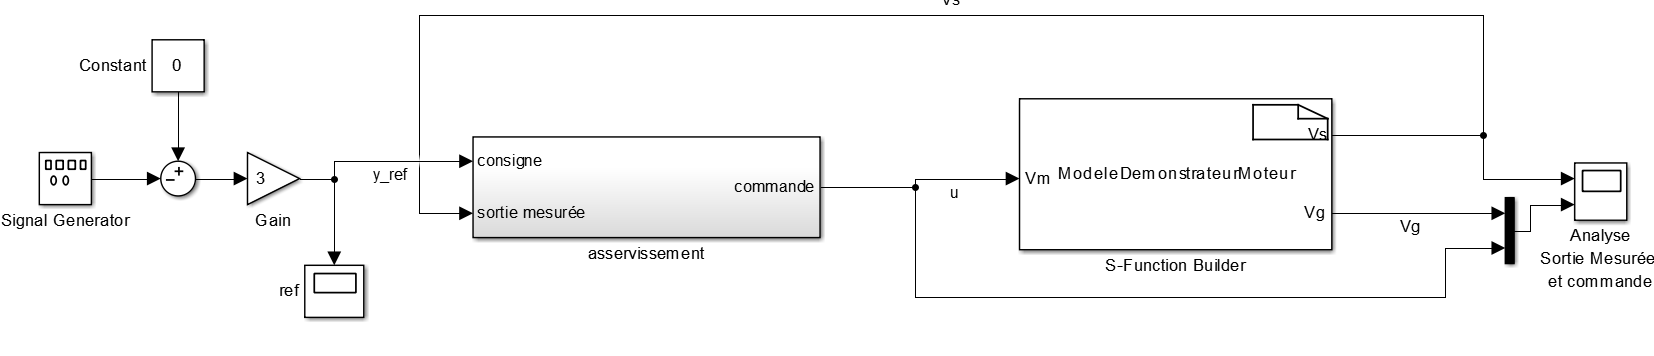
\includegraphics[width = \textwidth]{./annexes/annexe3/NL_RE_BlocEntier.png}
\caption{Schéma \emph{SIMULINK} complet de l'asservissement du modèle du moteur Non linéaire\label{fig:SIMULINK_NL_schema}}
\end{figure}

\begin{figure}
\centering
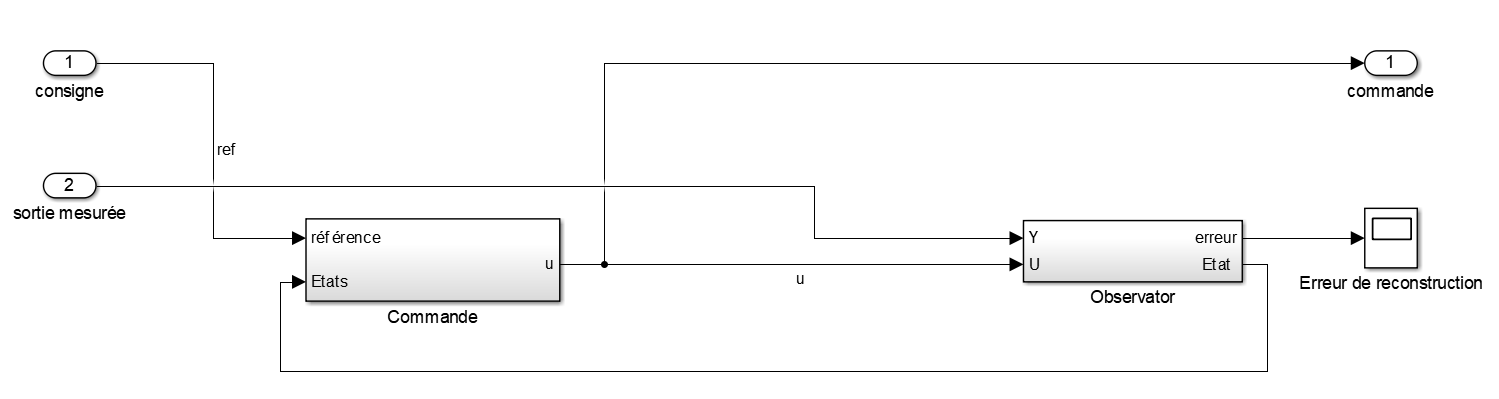
\includegraphics[width = \textwidth]{./annexes/annexe3/NL_RE_blocAsservissement.PNG}
\caption{Schéma \emph{SIMULINK} du \emph{sub-system} de commande\label{fig:SIMULINK_NL_subsystem_schema}}
\end{figure}

\begin{figure}
\centering
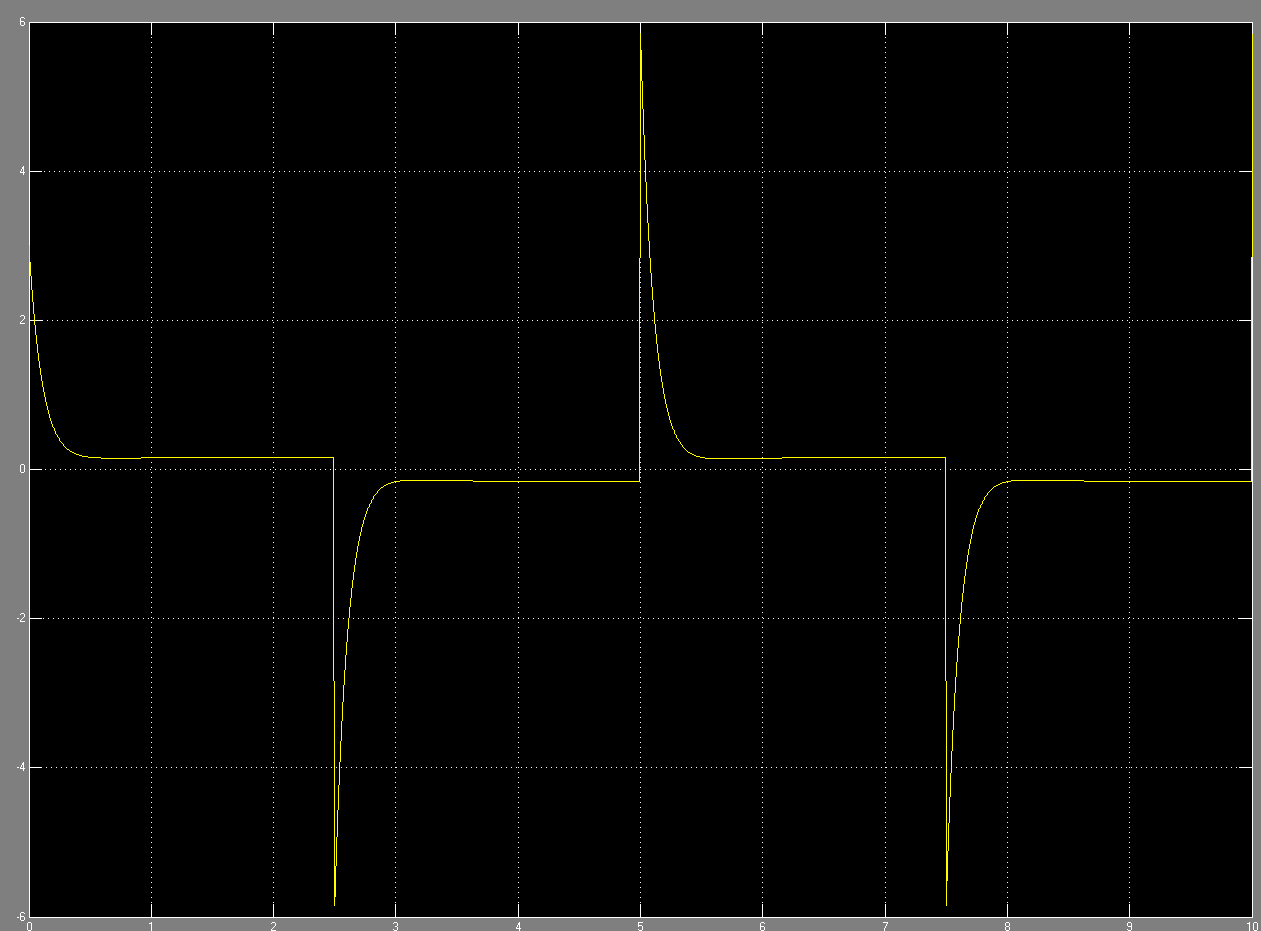
\includegraphics[width = .9\textwidth]{./annexes/annexe3/NL_erreur-Consigne_Vs_RE.png}
\caption{Mesure de simulation de l'erreur $\epsilon$ entre la référence et la sortie $V_s$ du modèle Non linéaire\label{fig:SIMULINK_NL_erreur_reponse}}
\end{figure}

\begin{figure}
\centering
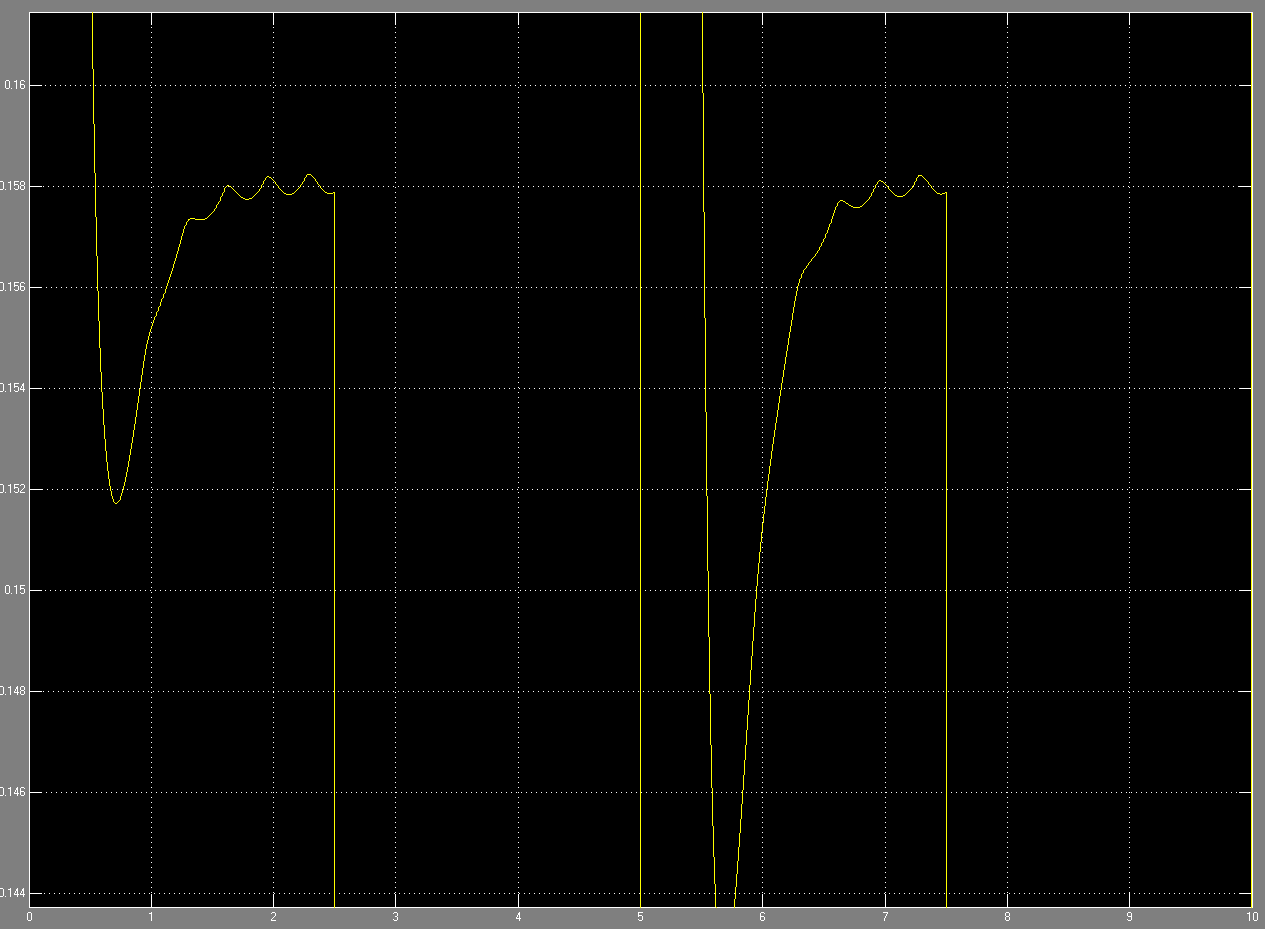
\includegraphics[width = .9\textwidth]{./annexes/annexe3/NL_erreur-Consigne_Vs_RE_zoom.png}
\caption{Mesure de simulation de l'erreur $\epsilon$ du modèle Non linéaire centré sur l'axe des ordonnées en $[0.144; 0.16].$\label{fig:SIMULINK_NL_erreur_reponse_zoom}}	
\end{figure}


>>>>>>> RapportChap4-2

	%


\newpage

%récupérer les citation avec "/footnotemark"
\nocite{*}

%%choix du style de la biblio
%\bibliographystyle{unsrt}
%%inclusion de la biblio
%\bibliography{bibliographie}
%%voir wiki pour plus d'information sur la syntaxe des entrées d'une bibliographie

\end{document}

